% ============================================================
% BanglaMix -- IEEE-style single-file manuscript (pdfLaTeX)
% Compile: pdflatex main -> bibtex main -> pdflatex main x2
% No Unicode/Bengali text is used, so standard pdfLaTeX works.
% ============================================================
% Two-column IEEE conference format (matches conference_101719.tex).
\documentclass[conference]{IEEEtran}

\usepackage{amsmath,amssymb,amsfonts}
\usepackage{graphicx}
\usepackage{booktabs}
\usepackage{array}
\usepackage{multirow}
\usepackage{xcolor}
\usepackage{subcaption}
\usepackage{stfloats}
\usepackage{enumitem}
\usepackage[hidelinks]{hyperref}
\usepackage{cite}
\usepackage{algorithm}
\usepackage{algpseudocode}
\usepackage{tikz}
\usetikzlibrary{positioning,arrows.meta}

\graphicspath{{figures/}}
\emergencystretch=2em

\definecolor{proposed}{RGB}{27,94,32}
\newcommand{\best}[1]{\textcolor{proposed}{\textbf{#1}}}

\begin{document}

\title{BanglaMix: A Dataset and Benchmark for Code-Switching {ASR}
in Bangladeshi Regional Dialects}

\author{\IEEEauthorblockN{M. Mohaiminul Islam}
\IEEEauthorblockA{\textit{Department of Computer Science and Engineering} \\
\textit{Noakhali Science and Technology University} \\
Noakhali, Bangladesh \\
mohaiminul.islam@nstu.edu.bd}}

\maketitle

\begin{abstract}
Automatic speech recognition (ASR) for low-resource, dialectal, and
code-switched speech remains an open problem. Existing Bengali resources
address either regional dialects or Bengali--English code-switching (CS), but
never both, even though young Bangladeshi speakers routinely mix English into
regional-dialect speech. This work introduces \textbf{BanglaMix}, the first
large-scale dataset for dialectal Bengali--English CS-ASR, comprising 41{,}499
transcribed clips (about 131 hours) spanning 15 regional dialects, collected from
social-media content where natural code-switching is most common. A fully
automated pipeline based on voice-activity segmentation, Whisper-based
silver-standard transcription, script-based code-switch detection, and a
single large language model (LLM) judge for borderline clips removes the need
for manual transcribers. Three ASR families are benchmarked under zero-shot and
fine-tuned conditions: Whisper, Meta MMS, and wav2vec2-XLS-R. A controlled
ablation over training subsets (dialect-only, code-switch-only, and combined)
isolates the contribution of each data type. The fine-tuned Whisper-small model
reaches a word error rate (WER) of 0.80 and a character error rate (CER) of
0.49, a 25\% relative WER reduction over its zero-shot counterpart and a
statistically significant improvement ($p<0.001$, paired bootstrap) over every
zero-shot baseline and a fine-tuned CTC model, including zero-shot
Whisper~large-v3.
Absolute error rates remain high because dialectal Bengali has no standardized
orthography and the labels are silver-standard; a human validation of 61 clips
quantifies the label quality at WER~0.70 / CER~0.39, and BanglaMix is therefore
positioned as a challenging, open benchmark for the community. The dataset and
full construction-and-evaluation code are publicly available\footnote{Dataset:
\url{https://huggingface.co/datasets/niloycste68/Bangali_local_dialect_ASR_HF_Dataset};
code: \url{https://github.com/niloycste/ASR-Bengali-Local-Dialect-}.} to support
future research.
\end{abstract}

\begin{IEEEkeywords}
Automatic speech recognition, Bengali ASR, code-switching, dialectal speech,
low-resource speech recognition, Whisper, large language model judge.
\end{IEEEkeywords}

% =====================================================================
\section{Introduction}
\IEEEPARstart{S}{peech} is the most natural interface to technology, yet
automatic speech recognition (ASR) quality is highly uneven across languages
and speaking styles. Two factors that strongly degrade ASR are \emph{dialectal
variation} and \emph{code-switching} (CS), the practice of mixing words from a
second language into an utterance. Both are pervasive in everyday Bangladeshi
speech: the country has many mutually distinct regional dialects, and younger,
educated speakers freely insert English words into dialectal Bengali, producing
utterances such as ``\textit{chatgaiya bhashay phone unboxing kortachi, honestly
speaking camera performance onek bhalo}'' (``unboxing a phone in the Chittagong
dialect; honestly speaking, the camera performance is very good'').

Despite this, existing Bengali speech resources cover only one phenomenon at a
time. Read-speech corpora such as OpenSLR-37~\cite{kjartansson2018bengali} target
standard Bengali; the Ben-10 corpus~\cite{ben10_2025} covers ten dialects but
contains no code-switching; and the MUCS shared task~\cite{mucs2021} provides
Bengali--English CS only in standard (Dhaka) Bengali. No dataset or model
addresses their \emph{intersection}---dialectal Bengali speech mixed with
English---which is precisely the dominant informal communication style.

Recognizing this kind of speech is hard for several compounding reasons, and
understanding them motivates the design choices made throughout this work.
\begin{itemize}[leftmargin=*]
\item \textbf{Acoustic divergence.} Regional dialects differ from standard
Bengali in vowel quality, consonant clusters, prosody, and vocabulary, so
acoustic models trained on standard Bengali generalize poorly.
\item \textbf{Two scripts in one utterance.} Code-switching forces the model to
move between Bengali and Latin scripts within a single utterance, which
monolingual recognizers cannot represent at all.
\item \textbf{Data scarcity.} Dialectal and code-switched speech is rare in
existing corpora, and paid transcription of 15 dialects is prohibitively
expensive for a low-resource language.
\item \textbf{No standardized orthography.} Dialect words and borrowed English
words have no single accepted spelling, so even a perfect transcription can be
``wrong'' under a strict word-level metric.
\end{itemize}
These four factors shape the dataset pipeline (which avoids manual transcription
and uses script-based code-switch detection), the model choice (which favors a
shared-vocabulary sequence-to-sequence model), and the evaluation (which
emphasizes character-level error and code-switch-specific metrics).

This work fills that gap; Fig.~\ref{fig:overview} gives an end-to-end overview of
the dataset construction, models, and evaluation. The main contributions are as
follows.
\begin{enumerate}[leftmargin=*]
\item \textbf{BanglaMix dataset.} The first large-scale dataset for dialectal
Bengali--English CS-ASR: 41{,}499 transcribed clips (about 131 hours) across 15
regional dialects, sourced from social media using dialect-name search queries.
\item \textbf{Automated, annotator-free pipeline.} An end-to-end pipeline using
voice-activity segmentation, Whisper-based silver-standard transcription,
script-based CS detection, and a single strong multilingual LLM judge for
borderline transcripts, enabling large-scale annotation without manual
transcribers.
\item \textbf{Systematic benchmark and ablation.} A controlled comparison of
three ASR families under zero-shot and fine-tuned conditions, with a training
subset ablation (dialect-only, CS-only, combined) that isolates the value of
each data type.
\item \textbf{Honest analysis.} A detailed error, per-dialect, and
code-switching analysis, with statistical significance testing, that
characterizes \emph{where} current models fail and establishes BanglaMix as a
hard open benchmark.
\end{enumerate}

The remainder of this paper is organized as follows. Section~\ref{sec:related}
reviews related work on Bengali, dialectal, and code-switching ASR and positions
this work against it. Section~\ref{sec:dataset} details the BanglaMix dataset
and its construction pipeline. Section~\ref{sec:models} describes the ASR models
and the fine-tuning procedure, and Section~\ref{sec:setup} presents the
experimental setup. Section~\ref{sec:results} reports the main results, and
Section~\ref{sec:analysis} provides an in-depth error, code-switching, ablation,
and case-study analysis. Section~\ref{sec:limitations} discusses limitations and
reproducibility, and Section~\ref{sec:conclusion} concludes with directions for
future work. Table~\ref{tab:notation} summarizes the notation used throughout.

\begin{figure*}[t]
\centering
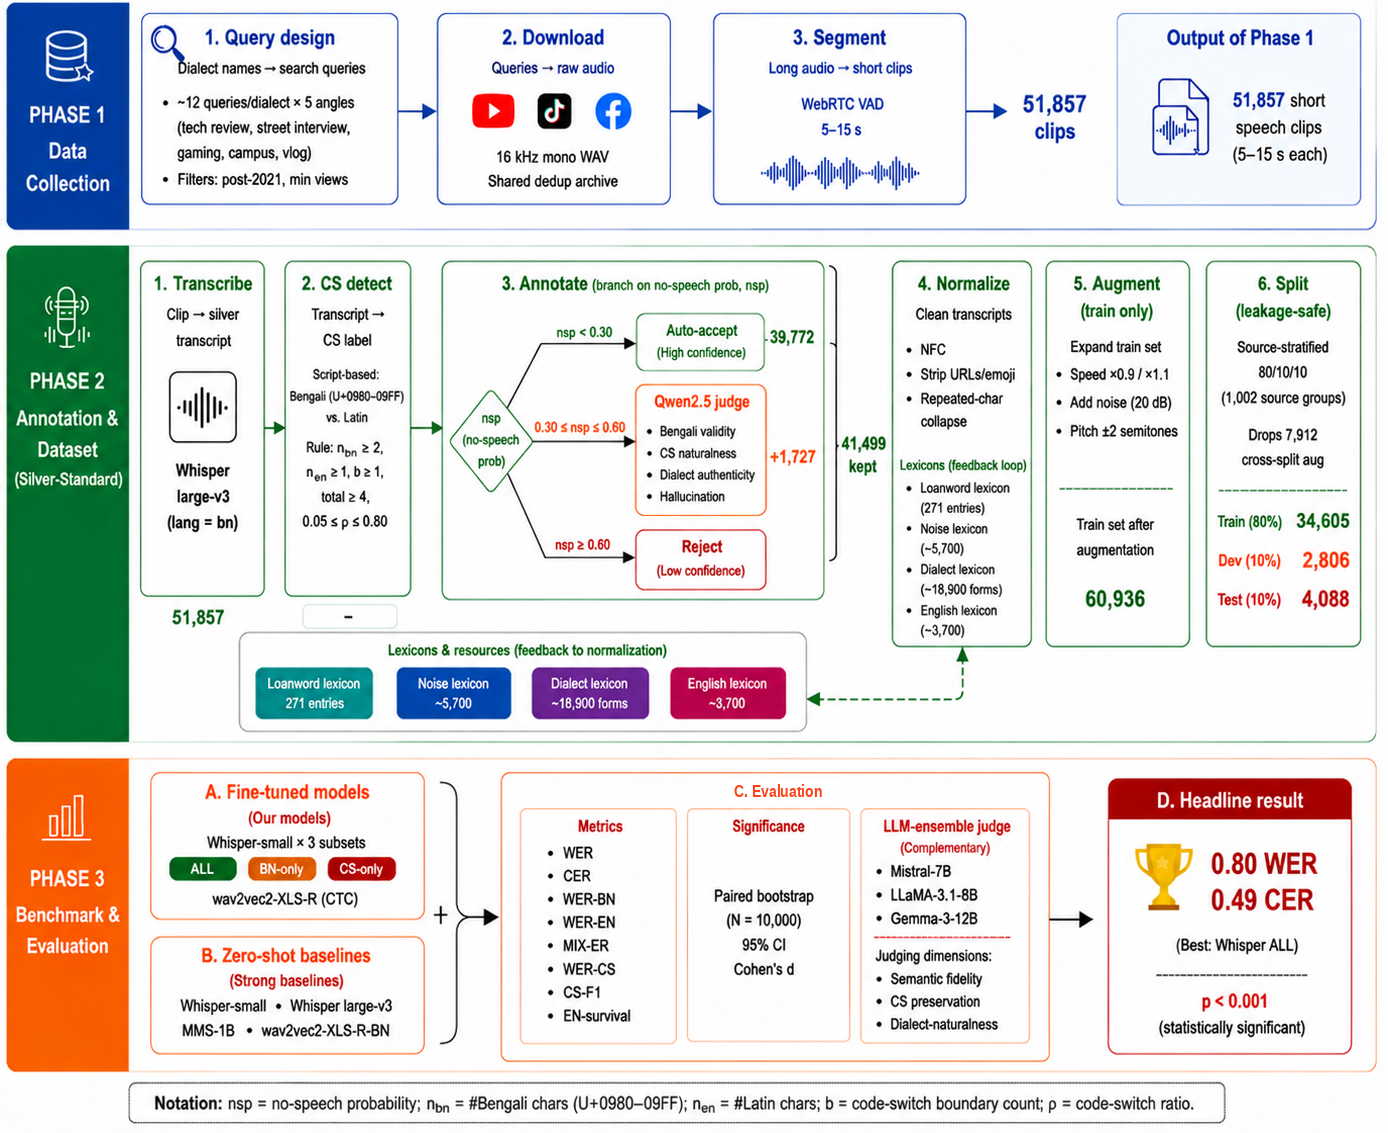
\includegraphics[width=\textwidth]{ASR_pipeline.png}
\caption{End-to-end overview of BanglaMix. Dialect-targeted social-media
collection and voice-activity segmentation feed a fully automated
silver-standard labeling stage (Whisper large-v3 transcription, script-based
code-switch detection, and an LLM judge), yielding 41{,}499 transcribed clips.
After normalization and a leakage-safe, source-stratified split, fine-tuned and
zero-shot ASR models are benchmarked with edit-distance, code-switching, and
LLM-ensemble metrics.}
\label{fig:overview}
\end{figure*}

\begin{table}[t]
\caption{Summary of notation.}
\label{tab:notation}
\centering\small
\begin{tabular}{ll}
\toprule
\textbf{Symbol} & \textbf{Description} \\
\midrule
$\tau_{\text{lo}},\tau_{\text{hi}}$ & low/high no-speech acceptance thresholds (0.30, 0.60) \\
$n_{\mathrm{bn}},n_{\mathrm{en}}$ & number of Bengali / English words in a clip \\
$b$ & number of intra-utterance language boundaries \\
$\rho$ & English-word ratio $n_{\mathrm{en}}/(n_{\mathrm{en}}+n_{\mathrm{bn}})$ \\
$S,D,I$ & substitutions, deletions, insertions in the alignment \\
$N$ & number of reference tokens \\
$\mathrm{P},\mathrm{R}$ & precision and recall of code-switch detection \\
$\mathcal{B}$ & CTC alignment-collapsing function \\
\bottomrule
\end{tabular}
\end{table}

% =====================================================================
\section{Related Work}
\label{sec:related}

\subsection{Bengali and Dialectal ASR}
Early Bengali ASR relied on Gaussian-mixture and deep-neural-network hidden
Markov models with hand-built pronunciation lexicons~\cite{hasnat2007isolated,
swarna2017survey}, which were limited to standard Bengali
and struggled with out-of-vocabulary words. The field then moved to end-to-end
models: connectionist temporal classification (CTC)~\cite{graves2006ctc}, deep
recurrent networks~\cite{graves2013speech}, Deep Speech~\cite{hannun2014deep},
and attention-based encoder--decoders such as Listen, Attend and
Spell~\cite{chan2016listen}, supported by toolkits such as
ESPnet~\cite{watanabe2018espnet}, which lowered error rates on standard
Bengali~\cite{mandal2020e2e}. The Transformer~\cite{vaswani2017attention} and
masked pre-training~\cite{devlin2019bert} subsequently enabled large
self-supervised and weakly-supervised speech models---wav2vec\,2.0
\cite{baevski2020wav2vec2}, HuBERT~\cite{hsu2021hubert}, WavLM~\cite{chen2022wavlm},
the multilingual XLS-R~\cite{babu2022xlsr,conneau2021xlsr},
Whisper~\cite{radford2023whisper}, and MMS~\cite{pratap2024mms}---which, together
with multilingual corpora such as Common Voice~\cite{ardila2020commonvoice},
improved transfer to low-resource Bengali. Dialectal Bengali received focused
attention only recently. The Ben-10 corpus~\cite{ben10_2025} covers ten regional
dialects (over 78 hours, 394 speakers) and shows that even strong foundation
models, including Whisper large-v3, perform poorly on out-of-distribution dialect
speech, both zero-shot and after fine-tuning. Biswas \emph{et al.}
\cite{biswas2025unified} propose a WavLM-based denoising and adaptation framework
for dialectal Bengali (e.g., Chittagonian and Sylheti) under simulated noise,
reporting large relative WER reductions over wav2vec\,2.0 and Whisper at low
signal-to-noise ratios. Ridoy \emph{et al.}~\cite{ridoy2025adaptability} compare
Whisper and Wav2Vec-BERT on standard Bangla and find the self-supervised encoder
both more accurate and more compute-efficient under low-resource conditions. None
of these, however, addresses code-switching, which motivates a benchmark that
combines dialect and code-switching in a single resource.

\subsection{Code-Switching ASR}
Code-switching---alternating between two languages within a conversation or even
a single utterance---is pervasive in multilingual societies and especially common
in informal Bangladeshi speech, where English words are routinely embedded in
Bengali sentences. It is hard for ASR for several compounding reasons: the
effective vocabulary spans two languages and, for Bengali--English, two scripts;
code-switched utterances are rare in standard training corpora; and language
switches interact with accent and acoustic variation, complicating both the
acoustic and language-modelling components~\cite{yilmaz2018augmentation,
sitaram2019survey}. Dedicated corpora have driven much of the progress in the
field, most prominently the Mandarin--English SEAME corpus~\cite{lyu2010seame},
while recent analysis shows that even large multilingual models handle
code-switching unreliably unless given explicit code-switched
supervision~\cite{winata2021multilingual}. For Indian languages, the MUCS~2021
challenge~\cite{mucs2021} introduced Bengali--English and Hindi--English
code-switching benchmarks, but its Bengali portion is restricted to standard
(Dhaka) Bengali and contains no regional dialects. A useful property of the
Bengali--English pair is that the two languages occupy disjoint Unicode ranges,
so word-level language identification is almost exact from script alone, without
a dedicated language-identification model. Architecturally, sequence-to-sequence
models such as Whisper are well suited to code-switching because their shared
sub-word vocabulary~\cite{sennrich2016bpe} already covers both scripts and can
emit mixed-script text in a single decoding pass, whereas monolingual CTC models
such as MMS must commit to one output script and cannot represent code-switching
at all. This work evaluates both paradigms in order to quantify that gap on
dialectal Bengali.

\subsection{Automated Corpus Construction for Low-Resource ASR}
Because manual transcription does not scale to many low-resource varieties,
recent corpora are built with automated pipelines. GigaSpeech~2
\cite{yang2025gigaspeech2} assembles a large multi-domain corpus for Thai,
Indonesian, and Vietnamese through automated web crawling, Whisper-based
transcription, and iterative refinement, demonstrating that weakly supervised
labels can replace human transcribers at scale. Complementary work uses synthetic
speech and spectrogram augmentation to enlarge low-resource training pools,
including for Bengali~\cite{dhahbi2025endtoend}. BanglaMix follows this automated
philosophy but targets a previously uncovered setting---multi-dialect Bengali
with English code-switching---and adds an LLM judge for borderline transcripts.

\subsection{LLM-as-a-Judge for Data Quality}
Using large language models (LLMs) as automatic evaluators has become common in
natural-language processing, ranging from pairwise response
judging~\cite{zheng2023judging,wang2023pandalm} to multi-dimensional quality
scoring~\cite{fu2023gptscore}. Such judges are attractive precisely when
human annotation is costly and reference labels are scarce or noisy---as in
low-resource dialectal ASR---although their reliability depends on prompt design
and the capacity of the judging model. In this work an LLM judge is used at two
distinct stages. During \emph{dataset construction}, a single strong multilingual
model (Qwen2.5~\cite{qwen2025}) scores borderline silver-standard transcripts
along several quality dimensions and decides whether to retain them. During
\emph{evaluation}, an ensemble of three open models---Mistral
\cite{jiang2023mistral}, LLaMA~\cite{dubey2024llama}, and
Gemma~\cite{team2024gemma}---provides an auxiliary, reference-free signal that
complements word-level metrics (Section~\ref{sec:analysis}). Applying LLM judges
to both quality control and evaluation for code-switched, low-resource ASR has,
to the authors' knowledge, not been explored before.

\subsection{Positioning of This Work}
Table~\ref{tab:relwork} summarizes representative Bengali and code-switching
ASR resources along the dimensions most relevant to this work. Two gaps are
clear. Standard-Bengali corpora and models~\cite{hasnat2007isolated,
swarna2017survey,mandal2020e2e,kjartansson2018bengali} address neither
dialect nor code-switching. The dialectal corpus Ben-10~\cite{ben10_2025} covers
multiple dialects but no code-switching, while the MUCS task~\cite{mucs2021}
covers code-switching but only in standard Bengali. General multilingual models
\cite{babu2022xlsr,radford2023whisper,pratap2024mms} transfer to standard
Bengali but degrade sharply on dialects and, for monolingual CTC models, cannot
emit code-switched output at all. BanglaMix is the first resource to occupy the
intersection: \emph{multi-dialect Bengali with natural English code-switching}.

\begin{table*}[t]
\caption{Comparative summary of representative Bengali and code-switching ASR
resources and models. ``CS'' indicates code-switching support; ``--'' denotes
not applicable. BanglaMix is the first to combine multi-dialect Bengali with
English code-switching.}
\label{tab:relwork}
\centering\footnotesize
\renewcommand{\arraystretch}{1.3}
\begin{tabular}{@{}p{2.5cm}p{2.6cm}p{2.6cm}p{1.7cm}cp{1.0cm}p{3.4cm}@{}}
\toprule
\textbf{Work} & \textbf{Method / Model} & \textbf{Objective} & \textbf{Variety} & \textbf{CS} & \textbf{Hours} & \textbf{Key limitation} \\
\midrule
Hasnat et al.~\cite{hasnat2007isolated} & GMM-HMM & Isolated-word Bengali ASR & Standard BN & No & -- & Lexicon-dependent; WER $>$50\%; no OOV handling \\
Swarna et al.~\cite{swarna2017survey} & Survey (HMM/GMM/DNN) & Bengali phoneme recognition survey & Standard BN & No & -- & Survey; standard Bengali, no dialect or CS \\
Mandal et al.~\cite{mandal2020e2e} & End-to-end (CTC/attention) & Lexicon-free Bengali ASR & Standard BN & No & -- & Standard Bengali only; no dialect or CS \\
Kjartansson et al.~\cite{kjartansson2018bengali} & OpenSLR-37 corpus & Read-speech benchmark & Standard BN & No & 100 & Read speech; no dialect, no code-switching \\
MUCS~2021~\cite{mucs2021} & CS challenge corpus & Bengali--English CS-ASR & Standard BN & Yes & 16 & Standard Dhaka Bengali; no dialect \\
Ben-10~\cite{ben10_2025} & Whisper fine-tuning & Multi-dialect Bengali ASR & Dialectal BN & No & 78 & No code-switching \\
XLS-R~\cite{babu2022xlsr} & wav2vec2 self-supervised & Multilingual transfer & Multilingual & No & -- & Standard Bengali via transfer; no dialect/CS \\
Whisper~\cite{radford2023whisper} & Weakly-supervised seq2seq & Multilingual ASR & Multilingual & No & -- & $\sim$70\% WER on unseen Bengali dialects \\
MMS~\cite{pratap2024mms} & CTC with adapters & 1000+ language ASR & Multilingual & No & -- & Monolingual output; cannot emit code-switching \\
Ridoy et al.~\cite{ridoy2025adaptability} & Whisper vs.\ Wav2Vec-BERT & Low-resource Bangla model comparison & Standard BN & No & $\sim$90--100 & Standard Bangla only; no dialect or CS \\
Biswas et al.~\cite{biswas2025unified} & WavLM denoising + adaptation & Noise-robust dialectal Bengali ASR & Dialectal BN & No & $\sim$20 & Dialectal but no code-switching; noise-focused \\
GigaSpeech~2~\cite{yang2025gigaspeech2} & Automated crawl + transcribe + refine & Large-scale low-resource corpus & Th/Id/Vi & No & $\sim$30k & Not Bengali; no dialect or code-switching \\
\midrule
\textbf{BanglaMix (this work)} & \textbf{Dataset + Whisper/CTC benchmark} & \textbf{Dialectal Bengali--English CS-ASR} & \textbf{Dialectal BN} & \textbf{Yes} & \textbf{165} & First multi-dialect Bengali with code-switching \\
\bottomrule
\end{tabular}
\end{table*}

% =====================================================================
\section{The BanglaMix Dataset}
\label{sec:dataset}

\subsection{Design Principles and Why They Matter}
BanglaMix is built around three principles. First, \emph{dialectal authenticity}:
the audio must contain genuine regional dialect, not standard Bengali spoken by
someone from a region. This matters because region-name queries (for example,
``Chittagong vlog'') mostly retrieve people \emph{from} a region speaking
standard Bengali to a general audience; dialect-name queries instead surface
content where creators deliberately use the dialect. Second, \emph{natural
code-switching}: CS must arise spontaneously in informal speech rather than from
scripted content, because scripted CS does not reflect real acoustic and
lexical patterns. Third, \emph{scalability}: the pipeline must be fully
automated so the dataset can grow without paid transcribers, which is essential
for a low-resource language where annotation budgets are small.

\subsection{Query Design}
Search queries are the single most important lever for collecting authentic
dialectal code-switched speech, because they determine \emph{which} creators are
retrieved. As noted above, region-name queries surface standard-Bengali content,
so this work instead uses \emph{dialect-name} queries combined with content
genres in which spontaneous code-switching is most frequent. For each dialect,
around a dozen queries are designed across five content angles, summarized in
Table~\ref{tab:queries}. The rationale is that street-interview and live-reaction
content is spontaneous and cannot sustain a fake accent, technology and campus
content elicits English technical terms, and vlog content yields relaxed, mixed
informal speech. Quality filters exclude pre-2021 uploads and videos with
negligible viewership.

\begin{table}[t]
\caption{Content angles used to design dialect-name search queries, and why each
elicits authentic dialectal code-switching.}
\label{tab:queries}
\centering\small
\begin{tabular}{p{2.4cm}p{5.0cm}}
\toprule
\textbf{Content angle} & \textbf{Why it elicits dialectal CS} \\
\midrule
Technology / phone review & Forces English technical terms within dialect speech \\
Street interview / reaction & Spontaneous public responses; a fake accent cannot be sustained \\
Gaming / live stream & Live commentary with frequent English game terms \\
Campus / career & Academic and job English mixed into regional speech \\
Vlog / content creator & Relaxed informal speech with frequent CS \\
\bottomrule
\end{tabular}
\end{table}

\subsection{Construction Pipeline}
Algorithm~\ref{alg:pipeline} summarizes the end-to-end pipeline; each step is
justified below.

\begin{algorithm}[t]
\caption{BanglaMix: From Raw Dialectal Audio to a Curated CS-ASR Benchmark}
\label{alg:pipeline}
\small
\begin{algorithmic}[1]
\Require dialect-name queries $\mathcal{Q}$; VAD aggressiveness $a$;
no-speech thresholds $\tau_{\text{lo}}{=}0.30,\ \tau_{\text{hi}}{=}0.60$; split ratio $80/10/10$
\Ensure curated dataset $\mathcal{D}=(\mathcal{D}_{\text{tr}},\mathcal{D}_{\text{dev}},\mathcal{D}_{\text{te}})$
\Statex \textit{Step 1: Acquire and segment}
\State $\mathcal{A} \gets \textsc{Download16k}(\mathcal{Q})$ \Comment{yt-dlp + ffmpeg; shared dedup archive}
\State $\mathcal{C} \gets \textsc{VADSegment}(\mathcal{A}, a)$ \Comment{WebRTC VAD; 5--15\,s clips $\Rightarrow$ 51{,}857}
\Statex \textit{Step 2: Transcribe and detect code-switching}
\For{each clip $c \in \mathcal{C}$}
    \State $t_c \gets \textsc{WhisperLargeV3}(c,\ \text{lang}{=}\text{bn})$
    \State $c.\textsc{cs} \gets \textsc{ScriptCSDetect}(t_c)$ \Comment{Bengali vs.\ Latin Unicode ranges}
\EndFor
\Statex \textit{Step 3: Silver-standard annotation (no human transcribers)}
\State $\mathcal{A} \gets \{c : \textsc{nsp}(c) < \tau_{\text{lo}}\}$ \Comment{auto-accept $\Rightarrow$ 39{,}772}
\State $\mathcal{B} \gets \{c : \tau_{\text{lo}} \le \textsc{nsp}(c) < \tau_{\text{hi}}\}$ \Comment{borderline $\Rightarrow$ 8{,}712}
\For{each $c \in \mathcal{B}$}
    \State $d \gets \textsc{Qwen2.5Judge}(t_c)$ \Comment{4 dimensions; \textsc{accept}/\textsc{reject}/\textsc{uncertain}}
    \If{$d = \textsc{accept}$}
        \State $\mathcal{A} \gets \mathcal{A} \cup \{c\}$ \Comment{$+1{,}727$; reviewed pool $\Rightarrow$ 41{,}499}
    \EndIf
\EndFor
\Statex \textit{Step 4: Normalise transcripts}
\State $\forall c \in \mathcal{A}:\ t_c \gets \textsc{Normalise}(t_c)$ \Comment{surface clean + 271-entry variant lexicon}
\Statex \textit{Step 5: Augment (training pool only)}
\State $\mathcal{G} \gets \textsc{Augment}(\mathcal{A})$ \Comment{speed $\times0.9/\times1.1$, $+$noise (20\,dB), pitch $\pm2$}
\Statex \textit{Step 6: Quality filter and leakage-safe split}
\State $\mathcal{A} \gets \textsc{DropLowQuality}(\mathcal{A} \cup \mathcal{G})$ \Comment{drop corrupted/foreign-script $\Rightarrow$ 75{,}742}
\State $(\mathcal{D}_{\text{tr}},\mathcal{D}_{\text{dev}},\mathcal{D}_{\text{te}}) \gets \textsc{SourceStratSplit}(\mathcal{A},\ 80/10/10)$ \Comment{1{,}002 source groups}
\State $\mathcal{D}_{\text{tr}} \gets \mathcal{D}_{\text{tr}} \cup \textsc{PinAugToTrain}(\mathcal{G})$ \Comment{leakage guard drops 7{,}912 cross-split aug.}
\State \Return $\mathcal{D}$ \Comment{60{,}936 / 2{,}806 / 4{,}088 (train/dev/test)}
\end{algorithmic}
\end{algorithm}

\paragraph*{Step 1: acquisition and segmentation}
Audio is downloaded at 16~kHz mono using \texttt{yt-dlp}~\cite{ytdlp} from
social-media platforms (YouTube, TikTok, and Facebook), with a shared
de-duplication archive so the same video is never collected twice. Long recordings are segmented into 5--15\,s clips using
WebRTC voice-activity detection~\cite{webrtcvad}. Segmentation is necessary
because raw social-media audio contains long non-speech regions, and fixed 5--15\,s
clips match the input length that modern ASR models train on, which keeps
both transcription and fine-tuning efficient. This step yields 51{,}857 clips.

\paragraph*{Step 2: transcription and CS detection}
Each clip is transcribed with Whisper large-v3~\cite{radford2023whisper} with the
language forced to Bengali. Whisper large-v3 is chosen as the labeler because it
is the strongest openly available multilingual model and therefore the best
available proxy for a human transcriber on this hard data. Code-switching is
detected directly from Unicode script ranges: Bengali (U+0980--U+09FF) and Latin
(ASCII) occupy disjoint ranges, so word-level language identification is nearly
exact without a dedicated model. Let $n_{\mathrm{bn}}$ and $n_{\mathrm{en}}$ be the number of Bengali- and
Latin-script words in a clip, $b$ the number of language boundaries (adjacent
words of different scripts), and $\rho = n_{\mathrm{en}}/(n_{\mathrm{en}}+
n_{\mathrm{bn}})$ the English-word ratio. A clip is labeled code-switched when
\begin{equation}
(n_{\mathrm{bn}}{+}n_{\mathrm{en}}) \ge 4 \;\wedge\; n_{\mathrm{bn}} \ge 2 \;\wedge\;
n_{\mathrm{en}} \ge 1 \;\wedge\; b \ge 1 \;\wedge\; 0.05 \le \rho \le 0.80 .
\end{equation}
A stricter high-confidence subset additionally requires $n_{\mathrm{en}} \ge 2$
and $0.10 \le \rho \le 0.70$. The lower bound on $\rho$ excludes isolated
borrowed words and the upper bound excludes English-dominant clips, so that only
genuinely mixed utterances are tagged; the same rule is applied to model
hypotheses when computing code-switch detection F1.

\paragraph*{Step 3--4: silver-standard annotation with an LLM judge}
Manual transcription of dialectal CS speech at scale is infeasible, so a
two-stage silver-standard strategy is used. High-confidence transcripts
(Whisper no-speech probability below $0.30$) are accepted directly, following
evidence that high-confidence Whisper output is a usable training
signal~\cite{gandhi2023whisper}; clips above $0.60$ are rejected as noise. The
uncertain middle band is the hard case, and here a single strong multilingual
judge (Qwen2.5~\cite{qwen2025}) scores each transcript on Bengali validity,
code-switch naturalness, dialect authenticity, and absence of hallucination, and
returns accept/reject/uncertain. A single high-capacity judge is used at this
stage---rather than an ensemble---because the borderline set is large and a
single strong model offers the best quality-per-compute trade-off; running it
locally also avoids API cost and keeps the data private. After this stage,
41{,}499 clips remain.

\paragraph*{Step 5: normalization}
Transcripts are cleaned with Unicode NFC normalization, removal of zero-width
characters, URLs, hashtags, mentions and emoji, digit normalization, repeated
character collapse, and punctuation/whitespace cleanup. A second, evaluation-only
step maps spelling variants of borrowed English words to a single canonical form
using a curated lexicon of 271 entries (649 variant spellings). This is
important because dialectal Bengali has \emph{no standardized orthography} for
loanwords, so the same spoken word may be written several valid ways; without
this mapping, word error rate would be inflated by legitimate spelling
variation rather than genuine recognition errors. The pipeline additionally
maintains three supporting lexicons that encode dialect- and code-switch-specific
knowledge: a list of about 5{,}700 known ASR hallucination and noise tokens, used
to detect and remove corrupted transcripts; a list of about 18{,}900 valid
dialectal Bengali word forms that are explicitly \emph{protected} from being
normalized toward standard spellings, so genuine dialect vocabulary is preserved;
and a list of about 3{,}700 common English words that supports the script-based
identification of code-switched tokens. These lexicons make the otherwise generic
normalization sensitive to the two phenomena---regional dialect and
code-switching---that this dataset targets.

\paragraph*{Step 6--7: augmentation, quality filter, and leakage-safe split}
Audio augmentation (speed perturbation, additive noise, pitch shift) is applied
to the training pool to improve robustness to acoustic variation, complementing
spectrogram-level methods such as SpecAugment~\cite{park2019specaugment}. The data is
then split at the \emph{source} level---all clips from one original video stay
in one split---to prevent speaker and channel leakage, which would otherwise
inflate test scores. The split is dialect-stratified so every dialect appears in
all three partitions. Augmented clips inherit their source and are pinned to
training only when that source is in the training split, so augmentation never
leaks a source across splits.

\subsection{Statistics}
Table~\ref{tab:dialects} lists the 15 dialects and Fig.~\ref{fig:dist} shows the
clip distribution, which is intentionally broad but naturally imbalanced,
mirroring online content availability. Of the 51{,}857 segmented clips, 41{,}499
pass silver-standard annotation and constitute the released dataset;
Table~\ref{tab:splits} reports its train/dev/test splits.

\begin{table}[t]
\caption{Dialect coverage in the released dataset.}
\label{tab:dialects}
\centering\small
\begin{tabular}{lrr}
\toprule
\textbf{Dialect} & \textbf{Clips} & \textbf{Hours} \\
\midrule
Sylhet & 7{,}931 & 26.0 \\
Old Dhaka & 4{,}741 & 14.6 \\
Sandwip & 4{,}583 & 13.0 \\
Barishal & 3{,}259 & 11.0 \\
Chittagong & 2{,}993 & 9.1 \\
Khulna & 2{,}774 & 8.9 \\
Narail & 2{,}371 & 7.8 \\
Kishoreganj & 2{,}287 & 7.1 \\
Rangpur & 1{,}985 & 6.4 \\
Comilla & 1{,}847 & 6.1 \\
Narsingdi & 1{,}661 & 5.1 \\
Habiganj & 1{,}446 & 4.5 \\
Mymensingh & 1{,}369 & 4.1 \\
Noakhali & 1{,}140 & 3.6 \\
Tangail & 1{,}112 & 3.8 \\
\midrule
\textbf{Total} & \textbf{41{,}499} & \textbf{131.2} \\
\bottomrule
\end{tabular}
\end{table}

\begin{figure}[t]
\centering
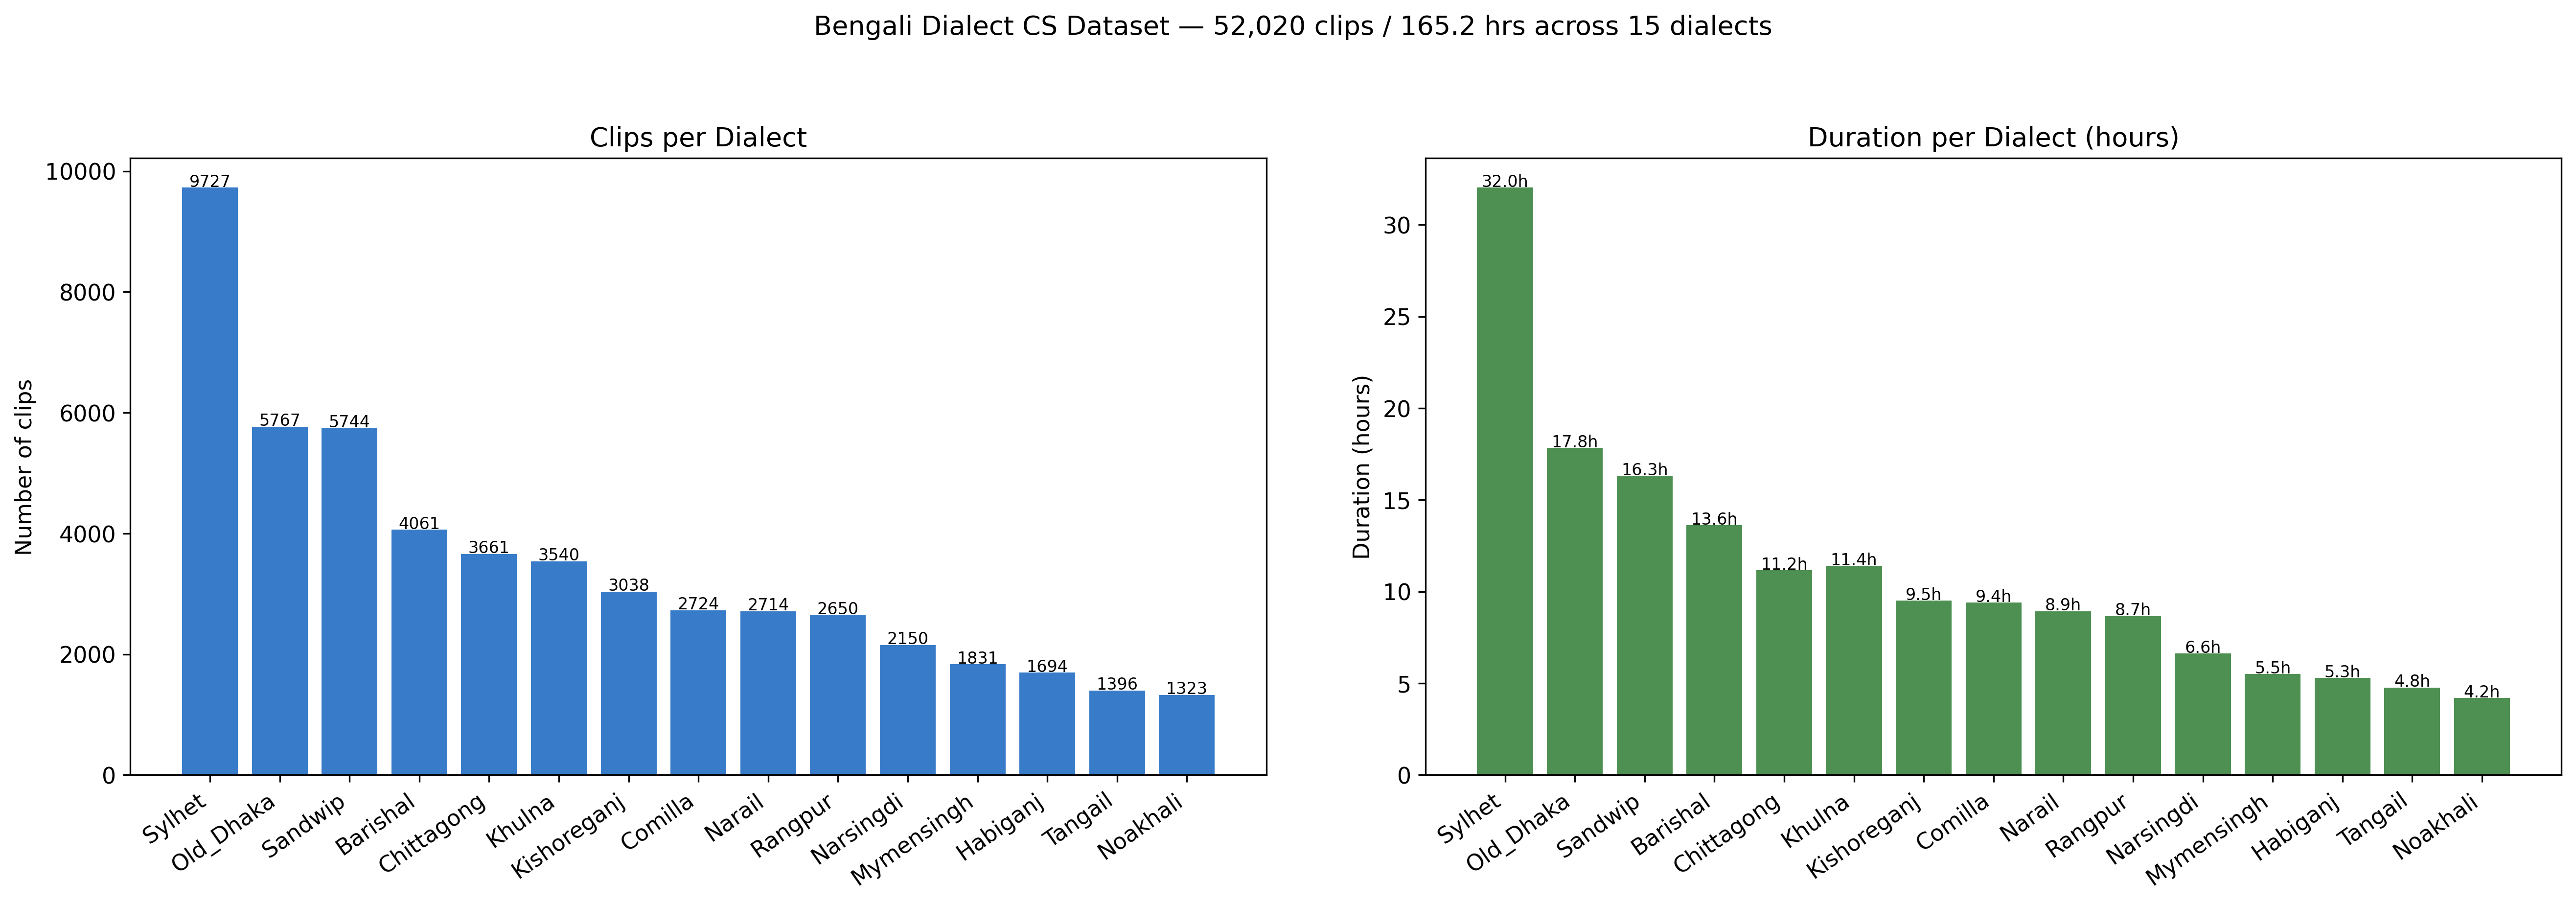
\includegraphics[width=\columnwidth]{dialect_distribution.png}
\caption{Clip distribution across the 15 dialects.}
\label{fig:dist}
\end{figure}

\begin{table}[t]
\caption{Train/dev/test splits of the released (real, unaugmented) dataset.
Audio augmentation expands the training split to 60{,}936 clips for model
training; dev and test remain real and unaugmented.}
\label{tab:splits}
\centering\small
\begin{tabular}{lrrrr}
\toprule
\textbf{Split} & \textbf{Clips} & \textbf{Hours} & \textbf{CS clips} & \textbf{CS\%} \\
\midrule
Train & 34{,}605 & 108.9 & 2{,}019 & 5.8 \\
Dev   & 2{,}806  & 9.1   & 166     & 5.9 \\
Test  & 4{,}088  & 13.2  & 176     & 4.3 \\
\midrule
Total & 41{,}499 & 131.2 & 2{,}361 & 5.7 \\
\bottomrule
\end{tabular}
\end{table}

\subsection{Human Validation of Silver-Standard Labels}
\label{sec:validation}
Because the transcripts are silver-standard, we quantify their reliability against
human reference. A bilingual annotator transcribed 61 randomly drawn test clips
(2--6 per dialect, balanced across the code-switching axis) by listening to the
audio; the human transcript is treated as the reference and the silver label as
the hypothesis. Overall agreement is \textbf{WER~$0.70$} and \textbf{CER~$0.39$}.
The large WER--CER gap is informative: at the character level the labels are far
closer to human transcription than the word-level figure suggests, reflecting the
absence of a standardized orthography for these dialects---annotators and Whisper
frequently choose different spellings of the same spoken word, which inflates WER
without indicating a semantic error.

Two patterns are consistent across the sample. First, code-switched labels are
\emph{more} reliable than Bengali-only ones (WER $0.58$ vs.\ $0.74$): the embedded
English tokens act as clear acoustic anchors that the transcription model captures
well. Second, label quality varies by dialect (Table~\ref{tab:validation}):
Sandwip, Kishoreganj, Sylhet, Khulna, and Old~Dhaka are transcribed reliably
(WER~$\le 0.54$, CER~$\le 0.34$), whereas Habiganj and Noakhali are weakest
(WER~$>1.0$, CER~$\approx 0.6$), driven by Whisper insertions and hallucination on
their more divergent phonology. These figures bound the silver-label noise floor,
contextualize the absolute error rates reported in Section~\ref{sec:results}, and
motivate label-refinement directions (e.g.\ judge-guided self-training) for future
work. Per-dialect estimates rest on small samples ($n=2$--$6$) and are therefore
indicative rather than definitive.

\begin{table}[t]
\caption{Human validation of silver-standard labels on 61 test clips (human
reference vs.\ silver hypothesis). Lower is better; $n$ is clips per dialect.}
\label{tab:validation}
\centering\small
\begin{tabular}{lrrr}
\toprule
\textbf{Dialect} & \textbf{$n$} & \textbf{WER} & \textbf{CER} \\
\midrule
Sandwip     & 3 & 0.26 & 0.10 \\
Kishoreganj & 5 & 0.46 & 0.25 \\
Khulna      & 3 & 0.53 & 0.32 \\
Old Dhaka   & 6 & 0.54 & 0.31 \\
Sylhet      & 4 & 0.54 & 0.34 \\
Narail      & 3 & 0.63 & 0.27 \\
Barishal    & 5 & 0.72 & 0.39 \\
Tangail     & 4 & 0.74 & 0.41 \\
Rangpur     & 6 & 0.75 & 0.51 \\
Narsingdi   & 3 & 0.76 & 0.38 \\
Chittagong  & 4 & 0.80 & 0.40 \\
Mymensingh  & 6 & 0.84 & 0.47 \\
Comilla     & 2 & 0.92 & 0.44 \\
Noakhali    & 3 & 1.04 & 0.59 \\
Habiganj    & 4 & 1.06 & 0.60 \\
\midrule
\textbf{Overall} & \textbf{61} & \textbf{0.70} & \textbf{0.39} \\
\bottomrule
\end{tabular}
\end{table}

\subsection{Ethical and Legal Considerations}
All audio is sourced from publicly available social-media content. To respect
creators and platform terms, the released dataset will distribute segmented audio
clips and transcripts for non-commercial research use, together with source
identifiers and timestamps so that the original content can be located and
attribution preserved. Because the data is conversational and may contain
personal opinions, no speaker identities, demographic labels, or contact
information are collected or released, and the dataset is intended only for
building and evaluating speech-recognition systems. Dialect coverage follows
online content availability rather than population, so it is intentionally not a
demographic sample; this imbalance is reported transparently
(Fig.~\ref{fig:dist}) so that downstream users can weight or resample as needed.

% =====================================================================
\section{ASR Models and Fine-Tuning}
\label{sec:models}
This work evaluates three model families, chosen to cover the two dominant ASR
paradigms and a range of pre-training regimes.

\paragraph*{Whisper (sequence-to-sequence)}
Whisper~\cite{radford2023whisper} is an encoder--decoder transformer trained on
680k hours of weakly supervised multilingual audio. It is central to this work
because its sub-word vocabulary contains both Bengali and Latin tokens, so it can
emit mixed-script (code-switched) output in a single decoding pass---a natural
fit for the task. While convolution-augmented architectures such as the
Conformer~\cite{gulati2020conformer} are also competitive for ASR, Whisper's
shared multilingual vocabulary makes it especially suited to code-switching.
The fine-tuned models use Whisper-small (244M parameters),
which is feasible to train on modest hardware while still benefiting from
large-scale pre-training. All inference forces Bengali transcription.

\paragraph*{Meta MMS (CTC, multilingual)}
MMS~\cite{pratap2024mms} is a CTC model covering 1{,}000+ languages with
per-language adapters. It is included as a strong multilingual zero-shot
baseline; because its output vocabulary is monolingual Bengali, it cannot emit
English script, which makes it a useful contrast for measuring how much
code-switching specifically hurts.

\paragraph*{wav2vec2-XLS-R (CTC, self-supervised)}
wav2vec2-XLS-R-300M~\cite{babu2022xlsr} is pre-trained on 436k hours of
multilingual audio. A Bengali-fine-tuned checkpoint is used as a zero-shot
baseline, and it is additionally fine-tuned on BanglaMix to represent the CTC
paradigm under the same training data as Whisper.

\paragraph*{Fine-tuning procedure}
Whisper is fine-tuned with the Hugging Face
Transformers~\cite{wolf2020transformers} and Datasets~\cite{lhoest2021datasets}
libraries using the Adam optimizer~\cite{kingma2015adam}: learning rate
$10^{-5}$, effective batch size 16, three epochs, 500 warm-up steps, with the
best checkpoint selected by development WER. For the CTC model, a character vocabulary
covering Bengali, Latin, and common punctuation is built from the training
transcripts, the CTC head is reinitialized, and the encoder is fine-tuned at
learning rate $10^{-4}$ for three epochs. All fine-tuning and benchmark
inference (zero-shot baselines and fine-tuned systems) run on a single
NVIDIA~A100-SXM4-40GB GPU, whereas the one-time silver-standard transcription of all clips
with Whisper~large-v3 was performed on a CPU workstation (Intel~Core~i9-14900,
24~cores, 32~GB RAM). The CTC model is trained to minimize
the negative log-likelihood marginalized over all alignments $\pi$ that collapse
to the target $y$,
\begin{equation}
\mathcal{L}_{\text{CTC}} = -\log \!\!\sum_{\pi \in \mathcal{B}^{-1}(y)} \prod_{t} p(\pi_t \mid x),
\end{equation}
where $\mathcal{B}$ is the CTC collapsing function, whereas Whisper is trained
with the standard token-level cross-entropy of its decoder. Key
hyperparameters are listed in Table~\ref{tab:hparams}. Fig.~\ref{fig:train}
shows that all
Whisper variants converge within about 2k steps; the CS-only ablation runs for
fewer steps because it uses only the roughly 4.5k code-switched clips.

\begin{figure}[t]
\centering
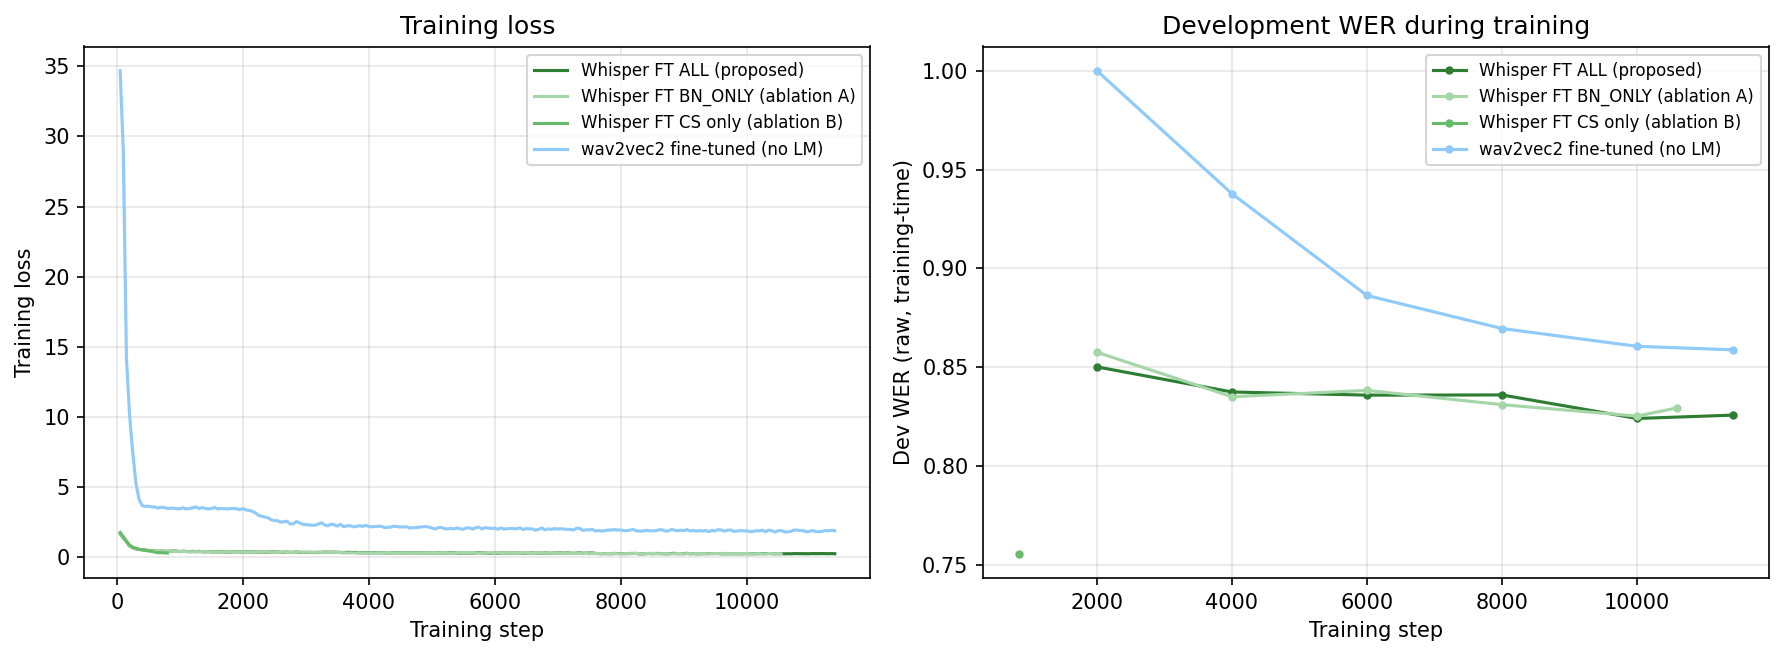
\includegraphics[width=\columnwidth]{training_curves.png}
\caption{Training loss (left) and development WER (right) during fine-tuning.
The development WER is the raw training-time value and is higher than the final
normalized test WER in Section~\ref{sec:results}.}
\label{fig:train}
\end{figure}

\begin{table}[t]
\caption{Fine-tuning hyperparameters for the two trained model families.}
\label{tab:hparams}
\centering\small
\begin{tabular}{lcc}
\toprule
\textbf{Hyperparameter} & \textbf{Whisper-small} & \textbf{wav2vec2-XLS-R} \\
\midrule
Base parameters & 244M & 300M \\
Architecture & seq2seq & CTC \\
Learning rate & $10^{-5}$ & $10^{-4}$ \\
Effective batch size & 16 & 16 \\
Epochs & 3 & 3 \\
Warm-up steps & 500 & 500 \\
Precision & bf16/fp16 & bf16/fp16 \\
Model selection & best dev WER & best dev WER \\
\bottomrule
\end{tabular}
\end{table}

\paragraph*{Training subset ablation}
To isolate the contribution of each data type, three Whisper variants are
trained: \textbf{BN\_ONLY} (dialect-only clips), \textbf{CS\_ONLY}
(code-switched clips only), and \textbf{ALL} (both). All three share the same
base model, procedure, and test set, so any difference is attributable to the
training data composition.

% =====================================================================
\section{Experimental Setup}
\label{sec:setup}

\subsection{Metrics and Why Each is Used}
Word error rate (WER) and character error rate (CER) are reported. CER is given
prominence because, with no standardized dialectal orthography, word-level WER
over-penalizes valid spelling variants, whereas CER better reflects how well the
sounds are captured. WER is further decomposed into WER-BN and WER-EN (errors on
Bengali and English words) to localize failures, and a mixed-error rate (MIX-ER)
measures combined script handling. Code-switch detection F1 (CS-F1) measures
whether a model produces any code-switching at all. All references and
hypotheses pass the same normalization (Section~\ref{sec:dataset}), including
collapse of degenerate repetition, before scoring, using standard error-rate
implementations~\cite{jiwer,evaluate2022}.

Formally, with $S$, $D$, and $I$ the number of substitutions, deletions, and
insertions from the reference--hypothesis alignment and $N$ reference tokens,
\begin{equation}
\text{WER} = \frac{S+D+I}{N},
\end{equation}
computed at the word level. CER applies the same edit-distance formula at the
character level,
\begin{equation}
\text{CER} = \frac{S_c+D_c+I_c}{N_c},
\end{equation}
where the subscript $c$ denotes character counts; CER is more robust to
inconsistent dialectal spelling and is therefore the primary metric in this
work. WER-BN and WER-EN restrict the alignment to Bengali-script and
Latin-script reference words, respectively, while the mixed error rate (MIX-ER)
treats each token as a (word, script) pair and counts a token correct only when
both the word \emph{and} its language match, jointly penalizing recognition and
script errors. Code-switch detection treats ``does the hypothesis contain
code-switching'' as a binary decision; with $\mathrm{TP}$, $\mathrm{FP}$, and
$\mathrm{FN}$ the true positives, false positives, and false negatives against
the script-based CS label,
\begin{equation}
\mathrm{P} = \frac{\mathrm{TP}}{\mathrm{TP}+\mathrm{FP}}, \quad
\mathrm{R} = \frac{\mathrm{TP}}{\mathrm{TP}+\mathrm{FN}}, \quad
\text{CS-F1} = \frac{2\,\mathrm{P}\cdot\mathrm{R}}{\mathrm{P}+\mathrm{R}}.
\end{equation}
Finally, English-word survival quantifies code-switch fidelity as the fraction
of Latin-script reference words on code-switched clips that also appear in the
hypothesis,
\begin{equation}
\text{EN-Surv} = \frac{1}{|\mathcal{C}|}\sum_{(r,h)\in\mathcal{C}}
\frac{|\,\{w\in r : \mathrm{lat}(w)\}\cap h\,|}{|\,\{w\in r : \mathrm{lat}(w)\}\,|},
\end{equation}
where $\mathcal{C}$ is the set of code-switched reference--hypothesis pairs and
$\mathrm{lat}(w)$ is true for Latin-script words.

\subsection{Baselines}
Four zero-shot baselines are used: \emph{Whisper-small}, the same base model as
the proposed system evaluated untuned, which isolates the effect of fine-tuning
from model scale; \emph{Whisper large-v3}, the strongest openly available model;
\emph{MMS-1B}; and \emph{wav2vec2-XLS-R-BN}, a Bengali CTC model trained on
standard Bengali.

\subsection{Significance Testing}
A paired bootstrap~\cite{berg2012empirical} ($N{=}10{,}000$ resamples over test
clips) is used, computing corpus WER on each resample, together with 95\%
confidence intervals. The paired
design is appropriate because all models are evaluated on the identical test
set.

% =====================================================================
\section{Results}
\label{sec:results}
Table~\ref{tab:main} reports the main results and Fig.~\ref{fig:wer} visualizes
overall WER.

\begin{table*}[t]
\caption{Main results on the BanglaMix test set (lower is better except CS-F1).
\best{Bold green} marks the best overall system; ``--'' denotes a metric not
applicable to a monolingual CTC model.}
\label{tab:main}
\centering\small
\begin{tabular}{llrrrrrrr}
\toprule
& \textbf{Model} & \textbf{WER} & \textbf{CER} & \textbf{WER-BN} & \textbf{WER-EN} & \textbf{MIX-ER} & \textbf{WER-CS} & \textbf{CS-F1} \\
\midrule
\multicolumn{9}{l}{\textit{Zero-shot baselines}}\\
& Whisper-small      & 1.07 & 1.02 & 1.07 & 1.26 & 1.15 & 1.02 & 0.00 \\
& Whisper large-v3   & 0.91 & 0.76 & 0.92 & 1.08 & 0.98 & 0.80 & 0.14 \\
& MMS-1B             & 0.99 & 0.57 & 0.99 & 1.11 & --   & 0.94 & 0.04 \\
& wav2vec2-XLS-R-BN  & 0.96 & 0.62 & 0.96 & 1.03 & --   & 0.94 & 0.04 \\
\midrule
\multicolumn{9}{l}{\textit{CTC fine-tuned on BanglaMix}}\\
& wav2vec2           & 0.86 & 0.49 & 0.86 & 1.00 & 0.97 & 0.88 & 0.14 \\
\midrule
\multicolumn{9}{l}{\textit{Whisper fine-tuned on BanglaMix (ablation)}}\\
& BN\_ONLY (A)       & 0.80 & 0.49 & 0.80 & 1.00 & 0.94 & 0.82 & 0.01 \\
& CS\_ONLY (B)       & 0.88 & 0.55 & 0.89 & \textbf{0.76} & \textbf{0.82} & 0.81 & \textbf{0.28} \\
& \best{ALL (proposed)} & \best{0.80} & \best{0.49} & \best{0.80} & \best{0.93} & \best{0.91} & \best{0.82} & \best{0.19} \\
\bottomrule
\end{tabular}
\end{table*}

\begin{figure}[t]
\centering
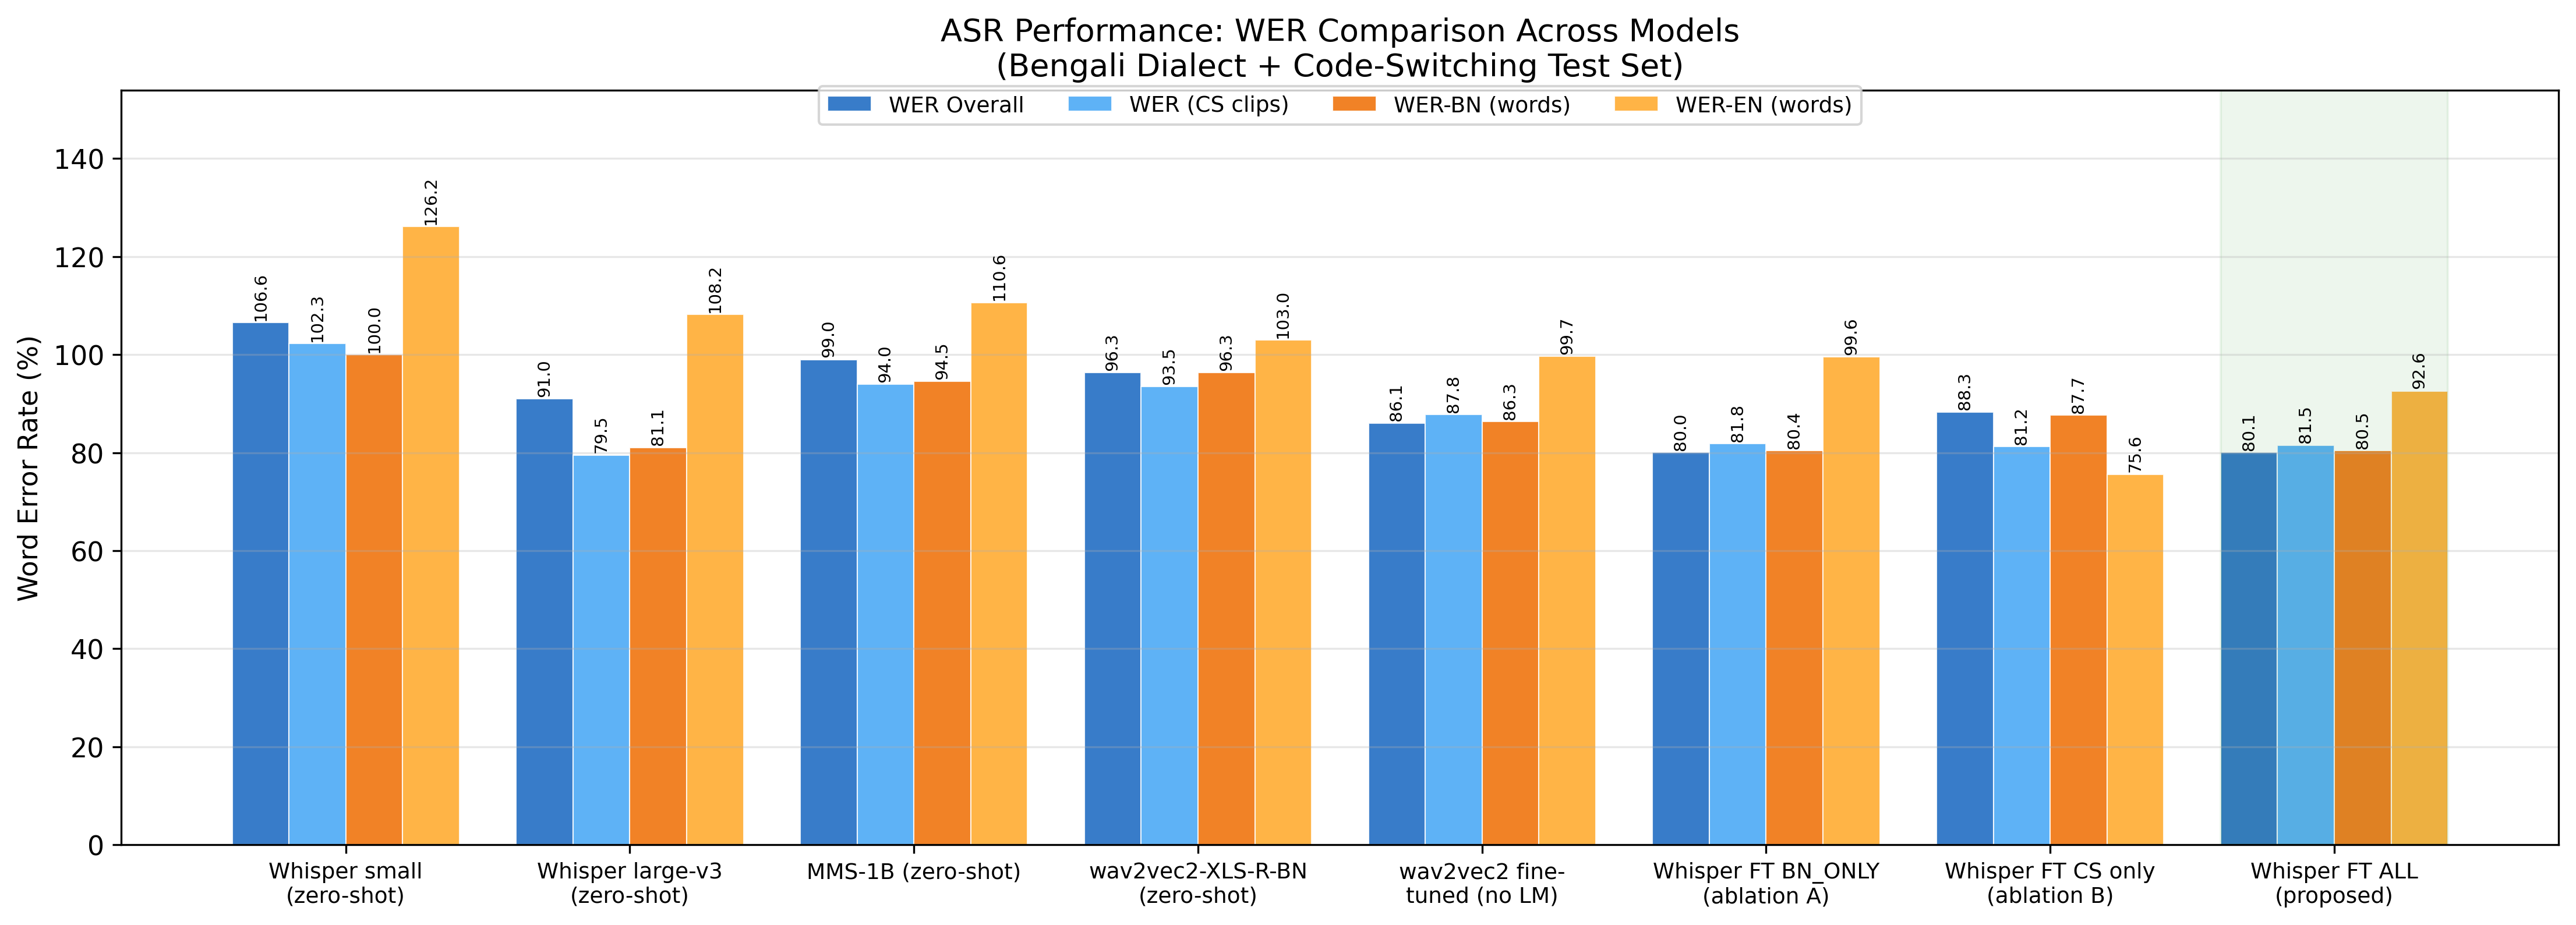
\includegraphics[width=\columnwidth]{wer_comparison.png}
\caption{Word error rate across all models. Fine-tuned systems are clearly
separated from zero-shot baselines.}
\label{fig:wer}
\end{figure}

\paragraph*{Zero-shot models fail on dialectal CS}
Whisper large-v3, despite 680k hours of pre-training, reaches only 0.91 WER, and
the same-size Whisper-small is worse (1.07 WER). Multilingual pre-training alone
does not transfer to dialectal code-switched Bengali.

\paragraph*{Fine-tuning helps substantially}
Fine-tuning Whisper-small on BanglaMix lowers WER from 1.07 to 0.80 and CER from
1.02 to 0.49---a 25\% relative WER reduction on an identical architecture, which
isolates the value of the data from model scale.

\paragraph*{The proposed model is strongest}
The ALL system attains 0.80 WER / 0.49 CER, significantly better than every
zero-shot baseline and the fine-tuned CTC model (0.86) at $p<0.001$ (paired
bootstrap; Section~\ref{sec:analysis})---for example, it improves on zero-shot
large-v3 (0.91). On overall WER it is statistically indistinguishable from the
BN-only ablation ($p{=}0.54$); as the ablation below shows, the value of training
on all data lies in code-switch handling rather than in overall WER.

\paragraph*{Ablation}
BN\_ONLY ties ALL on overall WER (0.80; difference not significant, $p{=}0.54$)
but barely recognizes English (CS-F1 0.01); CS\_ONLY best preserves English
(WER-EN 0.76, CS-F1 0.28) but sacrifices overall accuracy (0.88). Training on ALL
clips gives the best balance: overall accuracy on par with the best ablation
while substantially improving code-switch handling.

\subsection{Per-Dialect Results}
Table~\ref{tab:perdialect} reports per-dialect WER for the proposed system and
Fig.~\ref{fig:heatmap} shows the model$\times$dialect heatmap. The most
phonologically distinct dialect, Sylhet (27\% of the test set), is the hardest
across all models; central dialects (Khulna, Mymensingh, Narail, Noakhali) are
easiest.

\begin{table}[t]
\caption{Per-dialect WER/CER for the proposed Whisper ALL model.}
\label{tab:perdialect}
\centering\small
\begin{tabular}{lrrr}
\toprule
\textbf{Dialect} & \textbf{Clips} & \textbf{WER} & \textbf{CER} \\
\midrule
Sylhet & 1{,}111 & 0.93 & 0.65 \\
Old Dhaka & 360 & 0.78 & 0.53 \\
Sandwip & 176 & 0.92 & 0.67 \\
Barishal & 282 & 0.87 & 0.54 \\
Chittagong & 198 & 0.79 & 0.46 \\
Khulna & 120 & 0.66 & 0.39 \\
Kishoreganj & 743 & 0.75 & 0.36 \\
Comilla & 157 & 0.78 & 0.42 \\
Narail & 464 & 0.70 & 0.41 \\
Rangpur & 165 & 0.79 & 0.51 \\
Narsingdi & 60 & 0.72 & 0.39 \\
Mymensingh & 56 & 0.70 & 0.35 \\
Habiganj & 75 & 0.90 & 0.52 \\
Tangail & 51 & 0.74 & 0.39 \\
Noakhali & 70 & 0.70 & 0.36 \\
\midrule
\textbf{Overall} & \textbf{4{,}088} & \best{0.80} & \best{0.49} \\
\bottomrule
\end{tabular}
\end{table}

\begin{figure}[t]
\centering
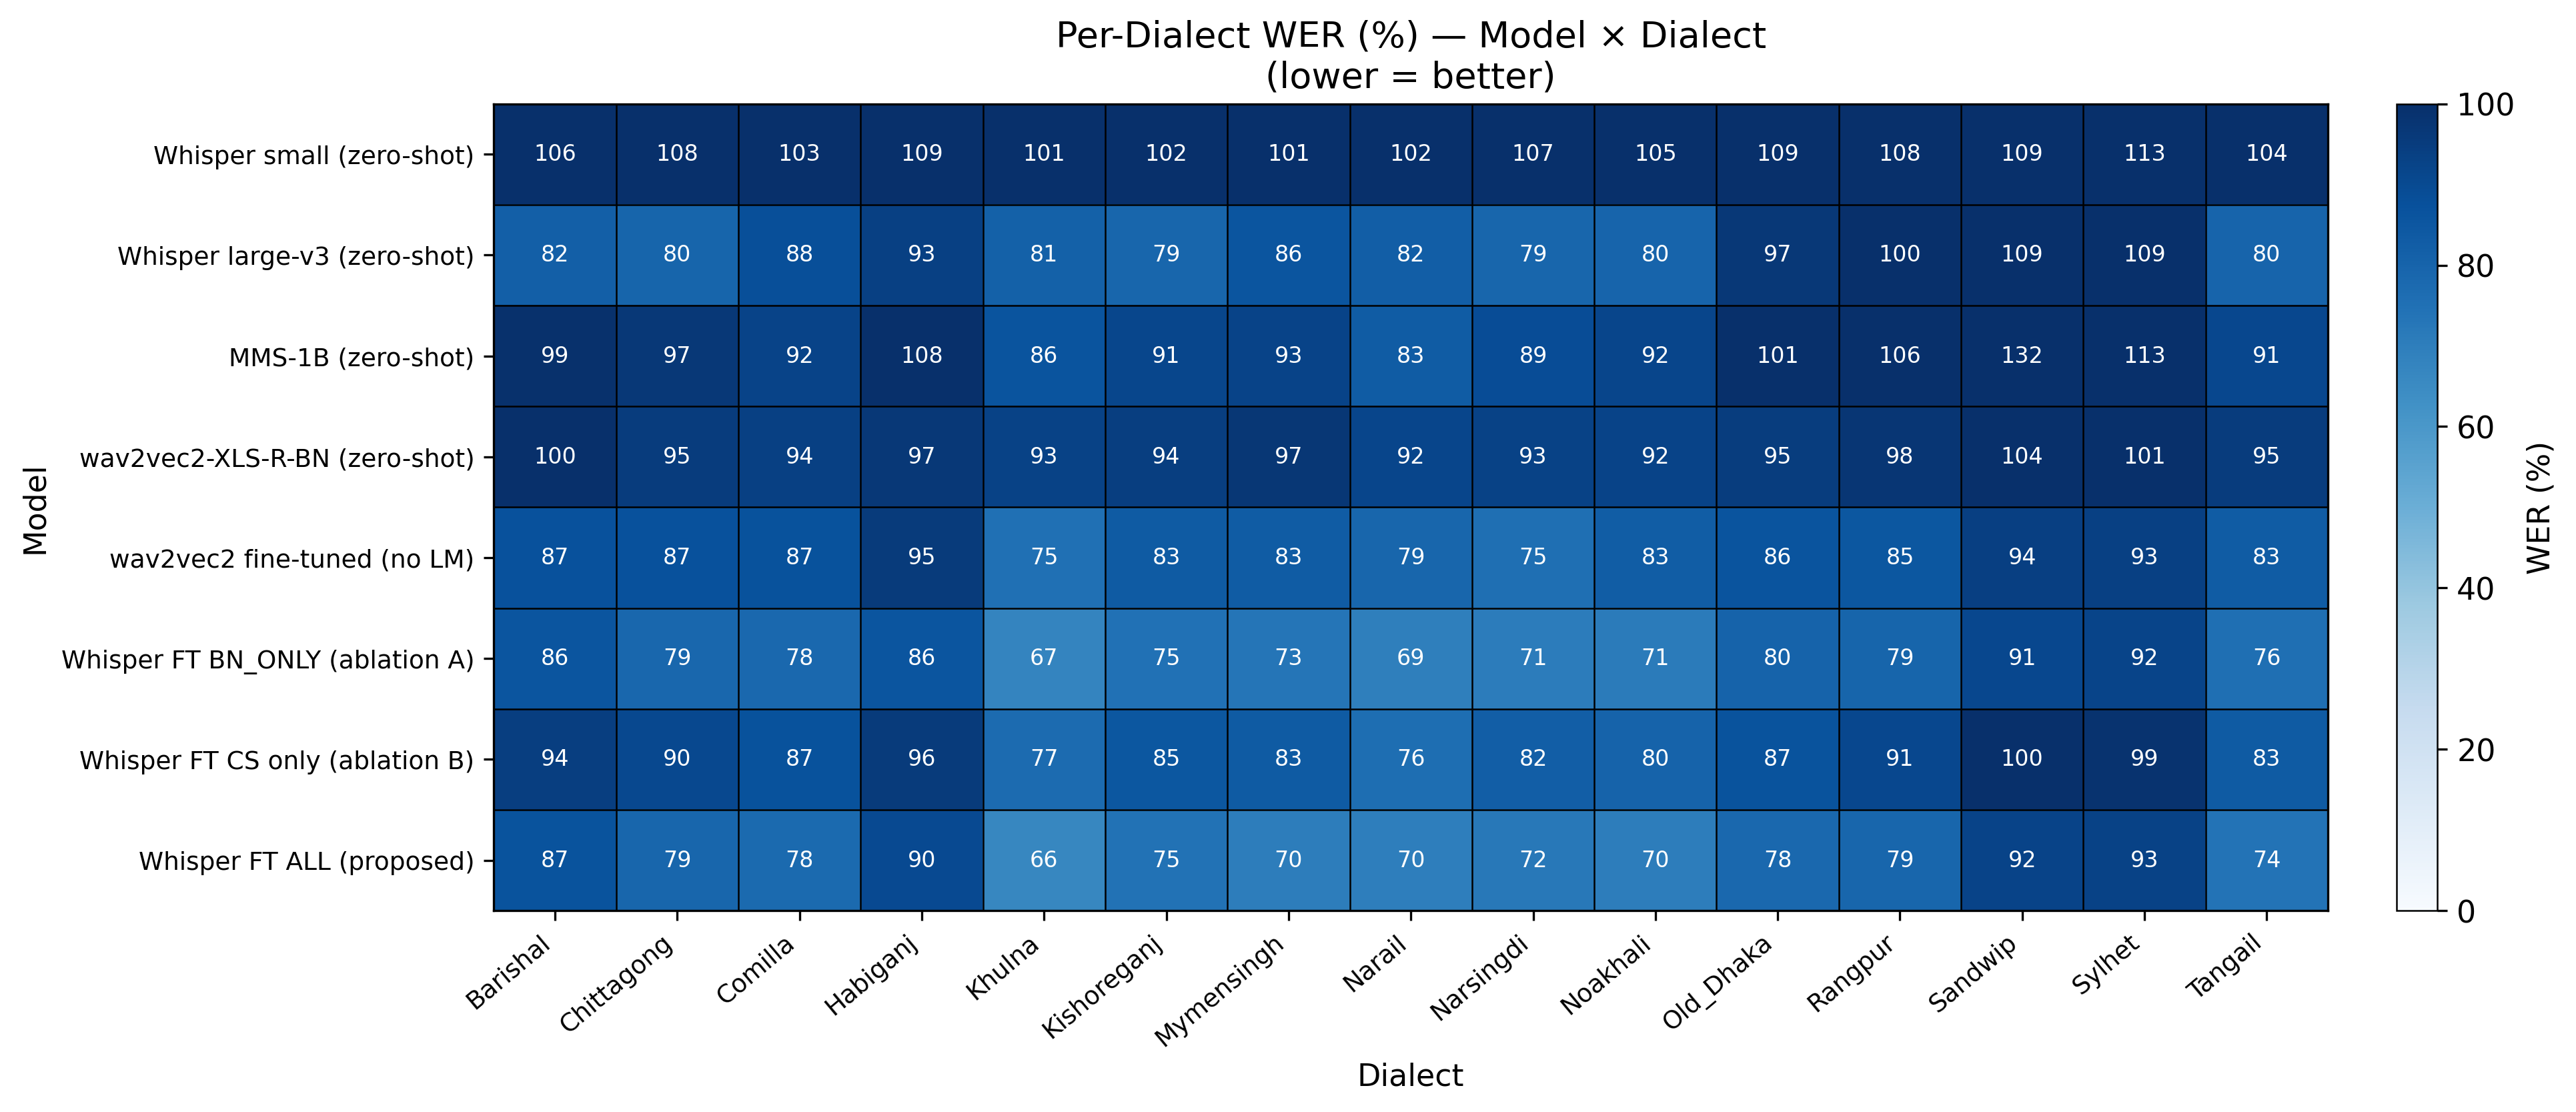
\includegraphics[width=\columnwidth]{dialect_wer_heatmap.png}
\caption{Model $\times$ dialect WER heatmap. Darker is higher WER.}
\label{fig:heatmap}
\end{figure}

Table~\ref{tab:cross} compares three representative models per dialect. The
proposed model is best or tied on 14 of 15 dialects; only on Barishal does the
larger zero-shot Whisper large-v3 win, indicating that model scale still matters
for some dialects and motivating larger fine-tuned backbones as future work.

\begin{table}[t]
\caption{Per-dialect WER for representative models. \best{Bold green} = best per
dialect.}
\label{tab:cross}
\centering\small
\begin{tabular}{lrrr}
\toprule
\textbf{Dialect} & \textbf{large-v3 (zs)} & \textbf{wav2vec2 (FT)} & \textbf{Whisper ALL} \\
\midrule
Sylhet & 1.09 & 0.93 & \best{0.93} \\
Old Dhaka & 0.97 & 0.86 & \best{0.78} \\
Sandwip & 1.09 & 0.94 & \best{0.92} \\
Barishal & \best{0.82} & 0.87 & 0.87 \\
Chittagong & 0.80 & 0.87 & \best{0.79} \\
Khulna & 0.81 & 0.75 & \best{0.66} \\
Kishoreganj & 0.79 & 0.83 & \best{0.75} \\
Comilla & 0.88 & 0.87 & \best{0.78} \\
Narail & 0.82 & 0.79 & \best{0.70} \\
Rangpur & 1.00 & 0.85 & \best{0.79} \\
Narsingdi & 0.79 & 0.75 & \best{0.72} \\
Mymensingh & 0.86 & 0.83 & \best{0.70} \\
Habiganj & 0.93 & 0.95 & \best{0.90} \\
Tangail & 0.80 & 0.83 & \best{0.74} \\
Noakhali & 0.80 & 0.83 & \best{0.70} \\
\bottomrule
\end{tabular}
\end{table}

% =====================================================================
\section{Analysis and Discussion}
\label{sec:analysis}

\subsection{Error Types and English-Word Survival}
Table~\ref{tab:errors} breaks WER into substitution (S), deletion (D), and
insertion (I) rates, and reports English-word survival (EN-Surv), the fraction
of English reference words that appear in the hypothesis on CS clips.
Fig.~\ref{fig:err} visualizes the S/D/I breakdown.

\begin{table}[t]
\caption{Error-type rates and English-word survival (EN-Surv).}
\label{tab:errors}
\centering\small
\begin{tabular}{lrrrr}
\toprule
\textbf{Model} & \textbf{S} & \textbf{D} & \textbf{I} & \textbf{EN-Surv} \\
\midrule
Whisper large-v3 (zs) & 0.31 & 0.48 & 0.12 & \textbf{0.65} \\
Whisper-small (zs)    & 0.25 & 0.75 & 0.07 & 0.12 \\
MMS-1B                & 0.66 & 0.13 & 0.19 & 0.00 \\
wav2vec2 (zs)         & 0.52 & 0.36 & 0.08 & 0.00 \\
wav2vec2 (FT)         & 0.52 & 0.23 & 0.10 & 0.00 \\
Whisper BN\_ONLY      & 0.45 & 0.21 & 0.14 & 0.01 \\
Whisper CS\_ONLY      & 0.53 & 0.19 & 0.16 & 0.37 \\
\textbf{Whisper ALL}  & 0.45 & 0.21 & 0.14 & 0.13 \\
\bottomrule
\end{tabular}
\end{table}

\begin{figure}[t]
\centering
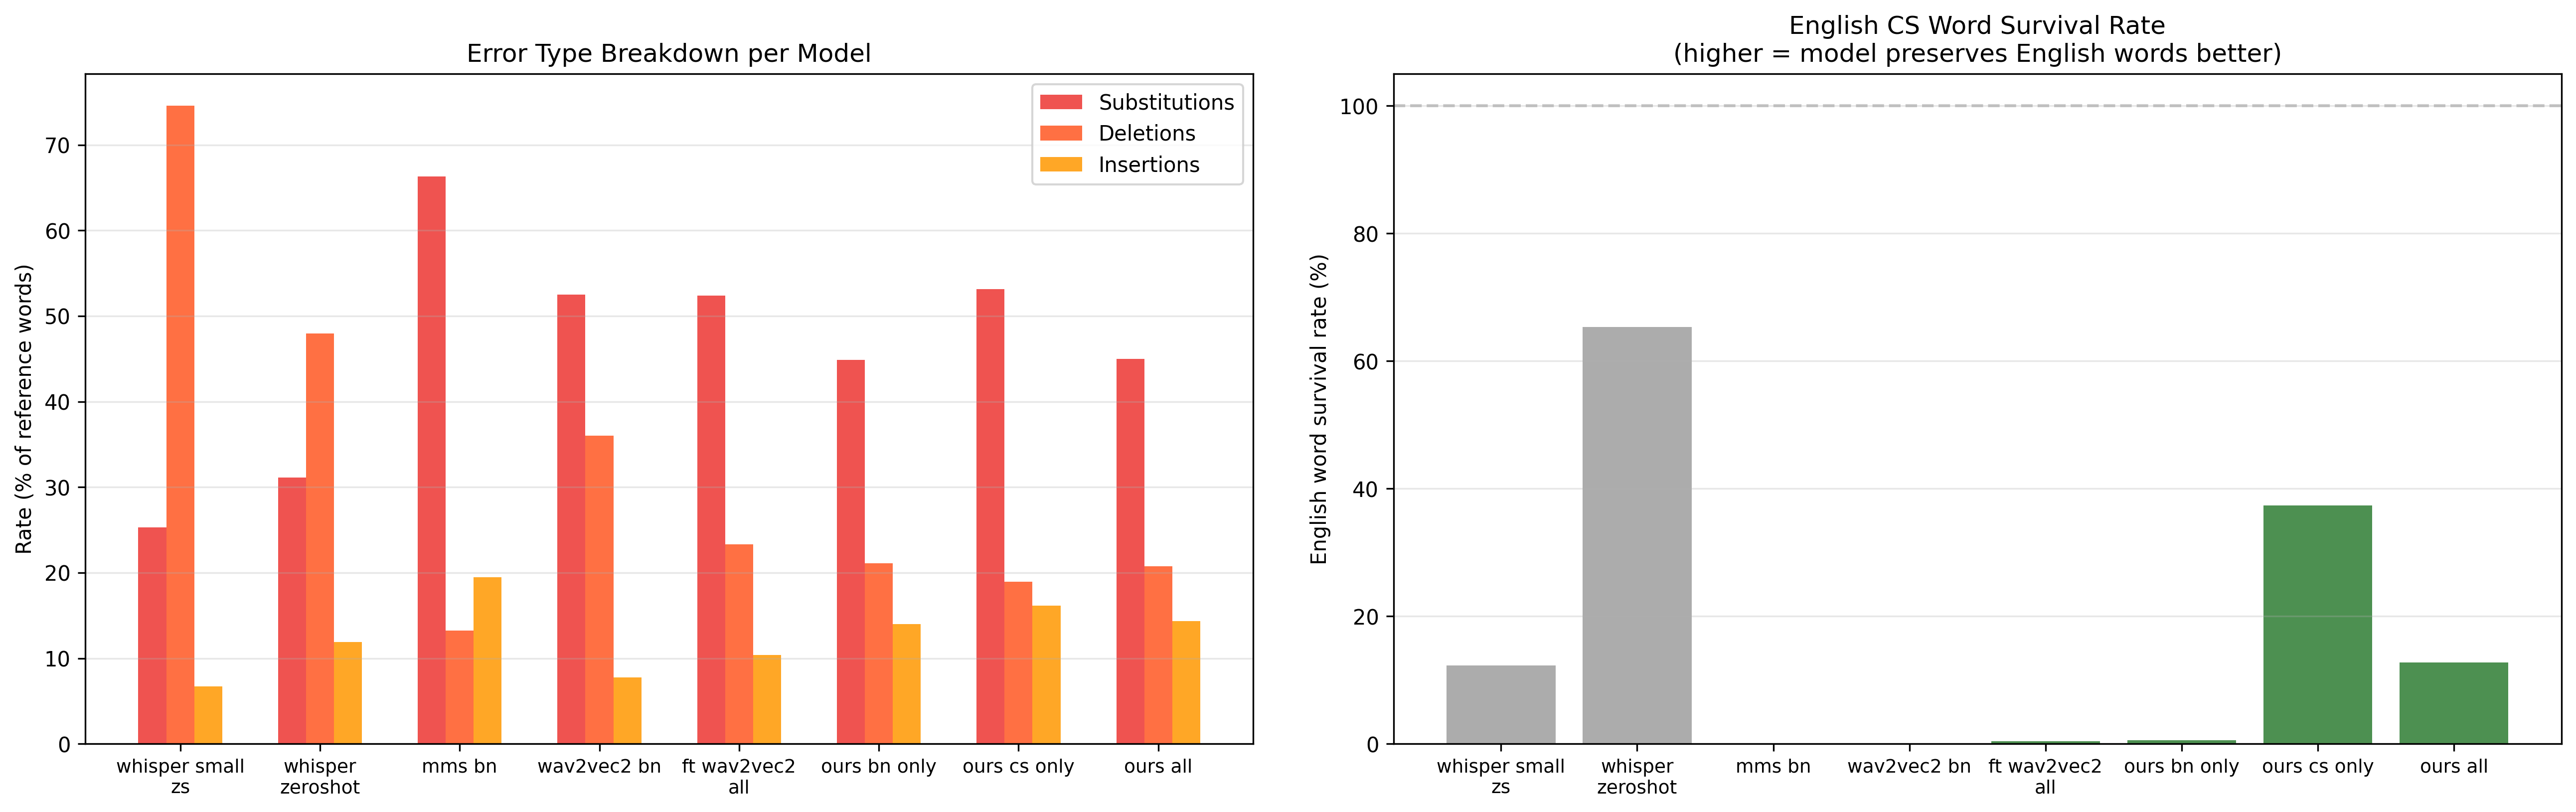
\includegraphics[width=\columnwidth]{error_analysis.png}
\caption{Substitution / deletion / insertion rates per model.}
\label{fig:err}
\end{figure}

A clear pattern emerges. Monolingual CTC models (MMS, wav2vec2) and the
Bengali-only ablation essentially never reproduce English words (EN-Surv at most
0.01): they delete English or map it to Bengali script. Code-switch training
raises this sharply---CS\_ONLY reaches 0.37, the best among fine-tuned models,
and ALL retains 0.13 while keeping the lowest overall WER. Zero-shot Whisper
large-v3 preserves English best of all (0.65) but at a far higher overall WER
(0.91), as it captures neither dialect phonology nor a coherent transcript. This
confirms that sequence-to-sequence models with a shared multilingual vocabulary,
fine-tuned on code-switched data, handle CS words far more faithfully than
monolingual CTC models.

\subsection{Where Code-Switching Difficulty Lives}
Table~\ref{tab:csgap} reports WER on CS versus Bengali-only clips. The whole-clip
gap is small (within $\pm0.12$): because CS clips are predominantly Bengali,
code-switching does not greatly change overall clip WER. The difficulty instead
lives in the English tokens themselves, as Table~\ref{tab:errors} shows---English
survival is near zero for monolingual and BN-only models. Fig.~\ref{fig:cs}
shows that models never trained on CS collapse to near-zero CS-F1, and that
training on code-switched data is what recovers code-switch behavior.

\begin{table}[t]
\caption{WER on CS vs.\ Bengali-only clips. Gap = WER-CS $-$ WER-BN.}
\label{tab:csgap}
\centering\small
\begin{tabular}{lrrr}
\toprule
\textbf{Model} & \textbf{WER-CS} & \textbf{WER-BN} & \textbf{Gap} \\
\midrule
Whisper large-v3 (zs) & 0.80 & 0.92 & $-$0.12 \\
Whisper-small (zs)    & 1.02 & 1.07 & $-$0.05 \\
MMS-1B                & 0.94 & 0.99 & $-$0.05 \\
wav2vec2 (FT)         & 0.88 & 0.86 & $+$0.02 \\
Whisper CS\_ONLY      & 0.81 & 0.89 & $-$0.08 \\
\best{Whisper ALL}    & \best{0.82} & \best{0.80} & \best{$+$0.02} \\
\bottomrule
\end{tabular}
\end{table}

\begin{figure}[t]
\centering
\begin{subfigure}{0.49\columnwidth}
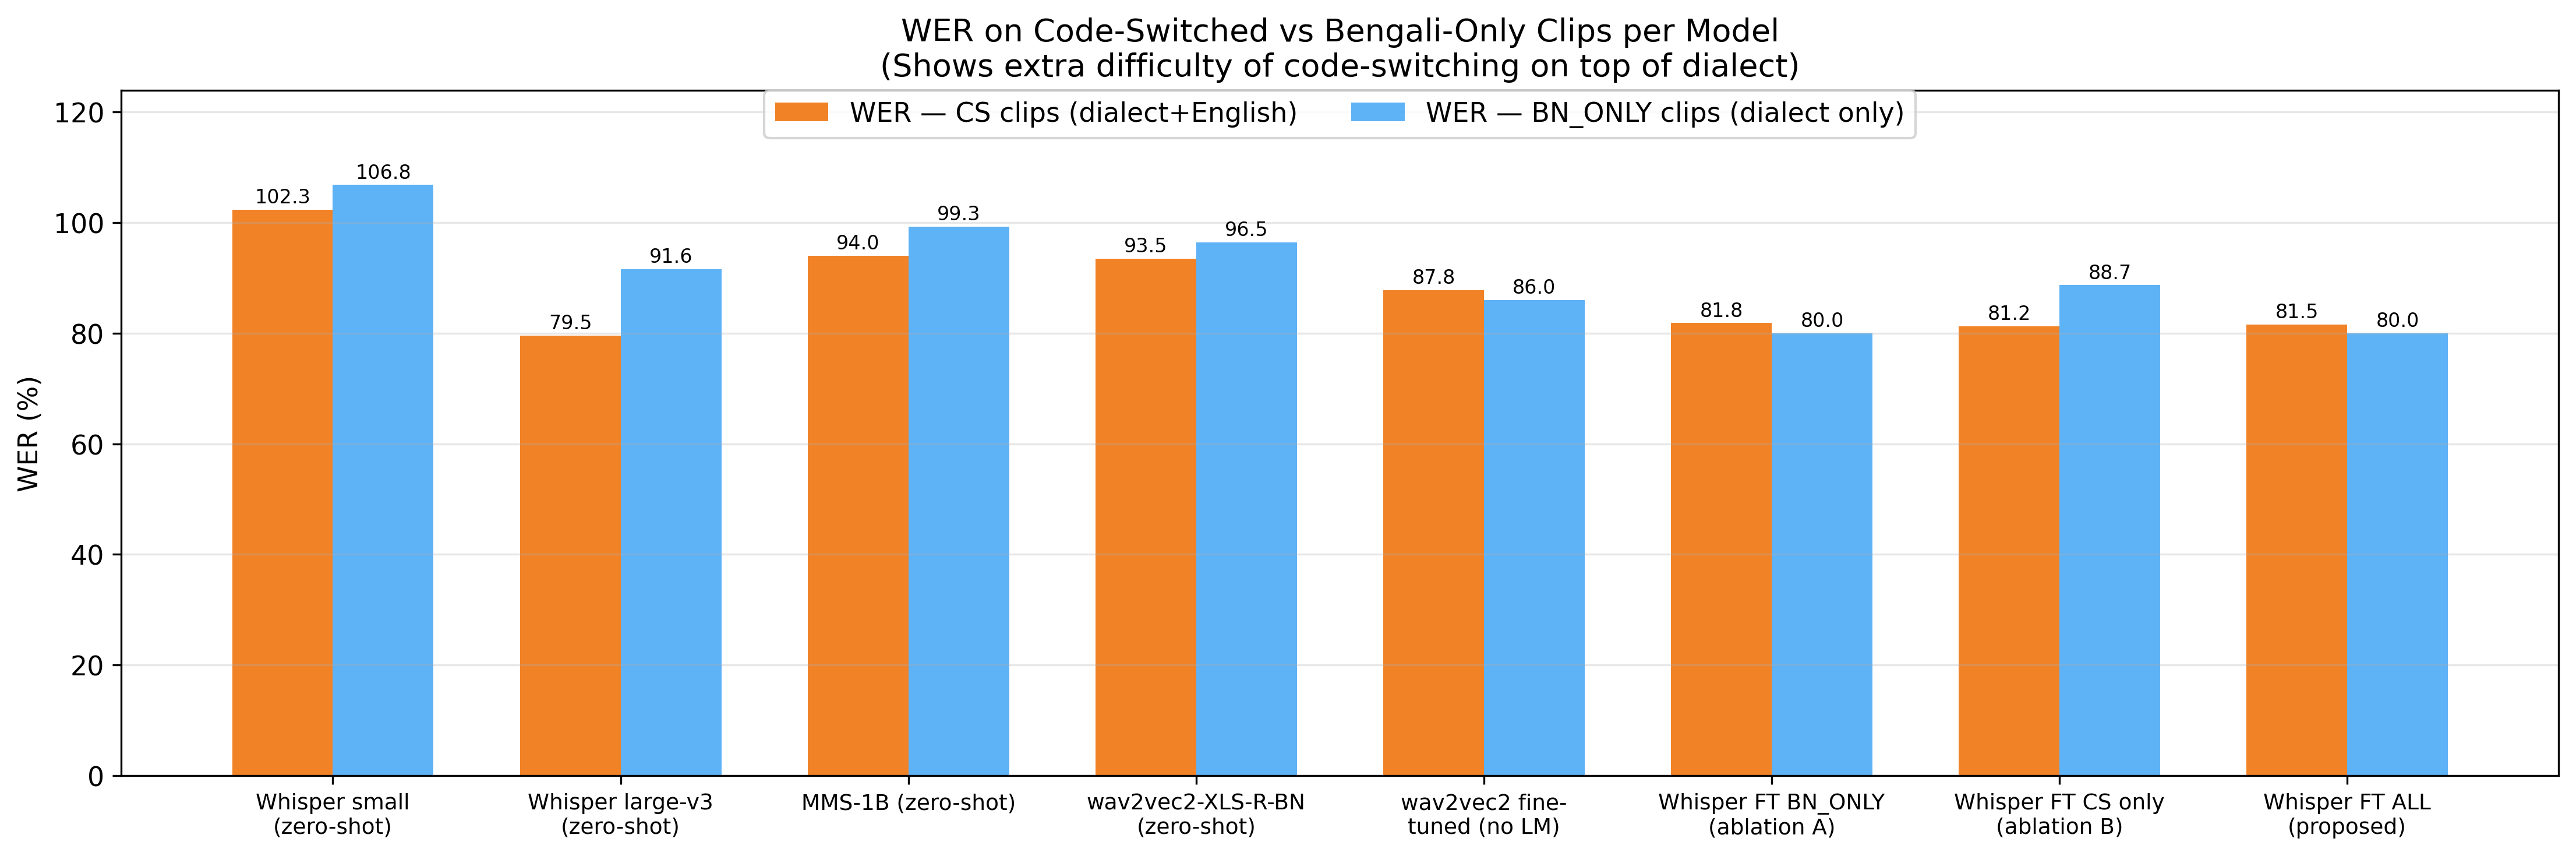
\includegraphics[width=\linewidth]{cs_vs_bn_wer.png}
\caption{WER: CS vs.\ BN clips.}
\end{subfigure}\hfill
\begin{subfigure}{0.49\columnwidth}
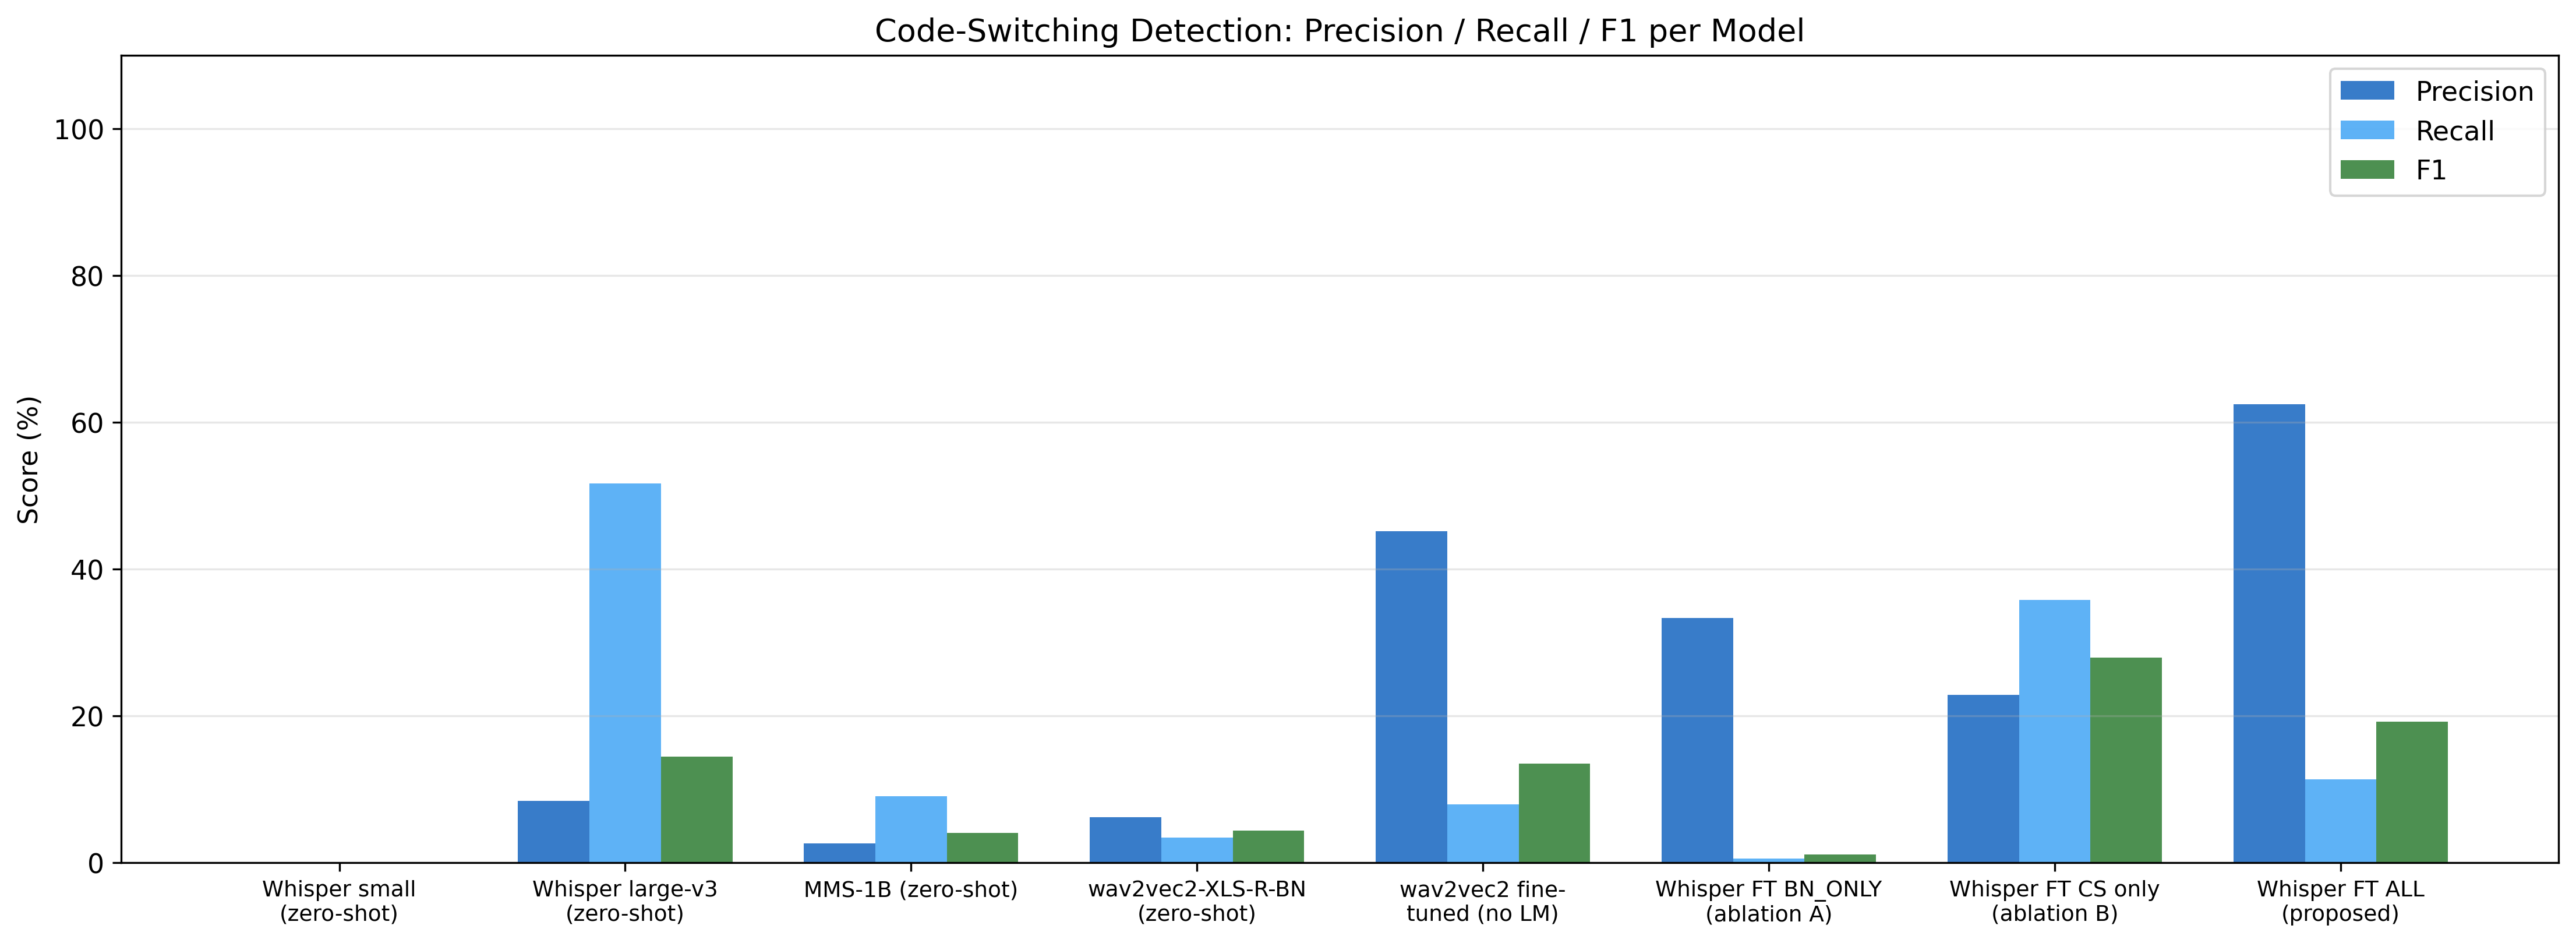
\includegraphics[width=\linewidth]{cs_f1_comparison.png}
\caption{Code-switch detection F1.}
\end{subfigure}
\caption{Code-switching analysis. Models never trained on CS show near-zero
CS-F1.}
\label{fig:cs}
\end{figure}

\subsection{Qualitative Error Analysis}
Inspecting model outputs reveals three recurring error patterns, illustrated
below with romanized examples (Bengali script omitted for readability).
\begin{itemize}[leftmargin=*]
\item \textbf{Repetition hallucination.} On out-of-distribution clips, zero-shot
Whisper enters degenerate loops, e.g.\ a one-word reference (``\textit{tai}'')
expands to forty repetitions of a single token. This pattern accounts for a
large share of the zero-shot insertion rate and is removed by the
repetition-collapse normalization before scoring.
\item \textbf{English deletion.} Monolingual and Bengali-only models drop English
words entirely: a reference ``\textit{ami office-e meeting korlam}'' is rendered
as ``\textit{ami $\dots$ korlam}'', omitting the English tokens. This is the
mechanism behind the near-zero English-word survival in
Table~\ref{tab:errors}.
\item \textbf{Spelling variance.} Fine-tuned models often produce a phonetically
correct but differently spelled form (e.g.\ ``\textit{kortasi}'' vs.\
``\textit{kortechi}'' for the same spoken word). These count as word errors yet
are not genuine recognition failures, which is precisely why CER is much lower
than WER and is the more faithful metric for this task.
\end{itemize}
These patterns explain the headline numbers: fine-tuning chiefly removes
hallucination and English deletion, while the residual error is dominated by
benign spelling variance over un-standardized dialectal orthography.

\subsection{Ablation Study}
Two ablations isolate key design choices. The \textit{training-subset} ablation
(Table~\ref{tab:main}) shows that BN\_ONLY and CS\_ONLY each sacrifice one
capability---BN\_ONLY collapses on English (CS-F1 0.01) while CS\_ONLY loses
overall accuracy (0.88 WER)---so only training on all data is strong on both.
The \textit{normalization} ablation (Table~\ref{tab:ablnorm}) isolates the
repetition-collapse step: applying it lowers the proposed model's WER from 0.96
to 0.80 and CER from 0.60 to 0.49 \emph{without changing the model}, by
preventing Whisper's degenerate decoding loops from dominating the score.

\begin{table}[t]
\caption{Effect of the repetition-collapse normalization on the proposed model
(model unchanged; scoring only).}
\label{tab:ablnorm}
\centering\small
\begin{tabular}{lcc}
\toprule
\textbf{Configuration} & \textbf{WER} & \textbf{CER} \\
\midrule
Without repetition collapse & 0.96 & 0.60 \\
\best{With repetition collapse (proposed)} & \best{0.80} & \best{0.49} \\
\bottomrule
\end{tabular}
\end{table}

\subsection{Case Study}
A single concrete case illustrates the dominant failure mode. On a short Sylheti
test clip whose reference is one word, zero-shot Whisper-small emits the same
token roughly forty times in a degenerate loop, producing an enormous per-clip
insertion count; the proposed fine-tuned model, decoded with repetition
collapse, instead returns a short hypothesis of the correct length. This case
explains both why zero-shot insertion rates are high (Table~\ref{tab:errors})
and why the normalization ablation (Table~\ref{tab:ablnorm}) yields such a large
apparent gain: a small number of pathological clips, rather than a uniform
degradation, drive much of the zero-shot error. The complementary failure on
code-switched clips is the deletion of English tokens by monolingual and
Bengali-only models, quantified by the near-zero English-word survival in
Table~\ref{tab:errors}.

\subsection{Statistical Significance}
All WER improvements of the proposed system over the four zero-shot baselines
and the fine-tuned CTC model are significant at $p<0.001$ (paired bootstrap,
$N{=}10{,}000$). The 95\% confidence interval for the proposed system's WER is
$[0.79,0.81]$, which does not overlap that of any baseline (for example,
zero-shot large-v3, $[0.90,0.92]$). The proposed model is \emph{not}
significantly different from the BN-only ablation on overall WER
($0.8009$ vs.\ $0.8004$, $p{=}0.54$); the two are equivalent on this metric, and
the benefit of training on all data instead appears in code-switch handling
(CS-F1 $0.19$ vs.\ $0.01$). Effect sizes against the baselines are statistically
robust but numerically small (Cohen's $d=0.09$ versus large-v3), as expected
when comparing models that all operate in a high-error regime on this
challenging benchmark.

\subsection{LLM-Ensemble Evaluation}
Word error rate captures surface accuracy but not whether a hypothesis is
\emph{semantically} faithful or preserves code-switching. As a complementary,
reference-free signal, an ensemble of three open LLMs
(Mistral-7B~\cite{jiang2023mistral}, LLaMA-3.1-8B~\cite{dubey2024llama},
Gemma-3-12B~\cite{team2024gemma}) scores each hypothesis from 0--5 on semantic
correctness, code-switch preservation, and dialect naturalness, on a stratified
50-clip sample per model. Table~\ref{tab:llmjudge} reports the means. The
proposed Whisper~ALL model attains the highest overall score (2.56/5), the best
semantic correctness (2.55), and the best code-switch preservation (2.71);
zero-shot large-v3 is marginally higher only on dialect naturalness
(2.57 vs.\ 2.43), and the CS-only ablation is lowest overall (2.21).
Inter-model agreement is 0.73--0.85. This corroborates the WER findings under an
independent, semantics-aware metric---the proposed model is judged best, and its
advantage is largest precisely on code-switch preservation---while the
mid-range absolute scores reflect the same task difficulty discussed above.

\begin{table}[t]
\caption{LLM-ensemble evaluation (mean score 0--5; three open judges; stratified
50-clip sample per model). \best{Bold green} = best per column.}
\label{tab:llmjudge}
\centering\small
\begin{tabular}{lcccc}
\toprule
\textbf{Model} & \textbf{Sem.} & \textbf{CS-pres.} & \textbf{Dialect} & \textbf{Overall} \\
\midrule
Whisper large-v3 (zs) & 2.41 & 2.46 & \best{2.57} & 2.48 \\
Whisper CS\_ONLY      & 2.27 & 2.32 & 2.05 & 2.21 \\
\best{Whisper ALL (proposed)} & \best{2.55} & \best{2.71} & 2.43 & \best{2.56} \\
\bottomrule
\end{tabular}
\end{table}

\subsection{Why Absolute Error Rates are High}
A WER near 0.80 is high relative to clean ASR (typically 0.05--0.20). Three
factors explain this and frame how the numbers should be read. First, the task
is intrinsically hard: 15 low-resource dialects combined with code-switching.
Second, dialectal Bengali has no standardized spelling, so word-level WER
penalizes valid spelling variants---which is why CER (0.49) is the more
informative metric here. Third, the reference labels are silver-standard
(generated by Whisper large-v3), so part of the measured error reflects label
noise rather than model failure. For these reasons BanglaMix is positioned as a
\emph{challenging open benchmark} rather than a solved task, and the relative,
statistically significant gains are the central result.

% =====================================================================
\section{Limitations}
\label{sec:limitations}
Several limitations frame the scope of this work and should guide interpretation
of the results. First, the transcripts are \emph{silver-standard}: they are
produced by Whisper large-v3 and validated by an LLM judge rather than by human
annotators, so part of the measured error reflects label noise. Our human
validation of 61 clips (Section~\ref{sec:validation}) bounds this noise at
WER~0.70 / CER~0.39 and shows it is uneven across dialects (WER~$0.26$--$1.06$);
because the silver labels originate from Whisper large-v3, the benchmark may also
slightly favour Whisper-family systems over other architectures, and a larger
human-validated subset remains valuable to tighten these per-dialect estimates.
Second, the fine-tuned
models use Whisper-small for tractability; larger backbones would likely lower
absolute error, as the per-dialect comparison already hints for dialects such as
Barishal. Third, code-switched clips are a minority ($\sim$6\%) of the data,
reflecting their natural prevalence; more aggressive query targeting could raise
this. Fourth, dialect coverage follows online content availability and is
imbalanced, with Sylhet dominating; as broader low-resource ASR surveys note,
such imbalance risks systematically under-serving speakers of less-represented
varieties, so per-dialect reporting and fairness-aware evaluation are
important~\cite{imam2025african}. Finally, the data is drawn from social-media
domains (vlogs, comedy, reviews) and may not transfer to formal domains such as
broadcast news, healthcare, or education.

\section{Reproducibility}
To support replication, the dataset (segmented clips, transcripts, and split
manifests) and the complete data and evaluation pipeline are publicly available
(see Data and Code Availability); the fine-tuned model checkpoints will be
released upon acceptance. All experiments are driven by a single
configuration file that fixes model identifiers, hyperparameters, and the
random seed used for the source-level split, so the train/dev/test partition is
deterministic. Evaluation applies the identical normalization to every model,
and the bootstrap significance test uses a fixed seed, so the reported
confidence intervals and $p$-values are reproducible from the prediction files.

% =====================================================================
\section{Conclusion}
\label{sec:conclusion}
This work introduced BanglaMix, the first large-scale dataset and benchmark for
dialectal Bengali--English code-switching ASR, together with a fully automated,
annotator-free construction pipeline. A systematic benchmark of three model
families shows that zero-shot multilingual models fail badly on this task,
that fine-tuning on BanglaMix yields large and statistically significant gains,
and that code-switching difficulty is concentrated in English tokens rather than
in overall clip error. The proposed fine-tuned Whisper model reaches 0.80 WER /
0.49 CER and outperforms every zero-shot baseline and the fine-tuned CTC model.
Absolute error remains high, reflecting un-standardized dialectal orthography and
silver-standard labels, so BanglaMix is released as an open benchmark to drive
further progress. Future work includes
larger fine-tuned backbones, a human-validated test subset, targeted data
collection for the hardest dialects such as Sylhet, and $n$-gram LM shallow
fusion for the CTC models using KenLM~\cite{heafield2011kenlm} and beam-search
decoding~\cite{pyctcdecode}. Language-model integration and tokenization tuned
specifically for dialectal Bengali, following recent low-resource LM-fusion
studies~\cite{dezuazo2025whisperlm,li2025contextual}, is a further promising
direction.

\section*{Data and Code Availability}
The BanglaMix dataset (segmented audio clips, silver-standard transcripts, and
train/dev/test split manifests) is publicly available on the Hugging Face Hub at
\url{https://huggingface.co/datasets/niloycste68/Bangali_local_dialect_ASR_HF_Dataset},
and the complete data-construction and evaluation code is available on GitHub at
\url{https://github.com/niloycste/ASR-Bengali-Local-Dialect-}. Both are released
for non-commercial research use to support reproducibility; the fine-tuned model
checkpoints will be released upon acceptance.

\section*{Declaration of Competing Interest}
The authors declare no known competing financial interests or personal
relationships that could have appeared to influence the work reported in this
paper.

\bibliographystyle{IEEEtran}
\bibliography{references}

\end{document}
